\documentclass[UTF8,a4paper,12pt]{ctexart}

\usepackage[top=2.5cm,bottom=2.5cm,left=2.5cm,right=2.5cm]{geometry}
\usepackage{amsmath,amssymb,bm}
\usepackage{graphicx}
\usepackage{booktabs}
\usepackage{multirow}
\usepackage{array}
\usepackage{float}
\usepackage{longtable}
\usepackage{caption}
\usepackage{subcaption}
\usepackage{enumitem}
\usepackage{hyperref}
\usepackage[strings]{underscore}
\usepackage{xcolor}
\usepackage{setspace}

\hypersetup{colorlinks=true,linkcolor=black,urlcolor=blue,citecolor=black}
\captionsetup{font=small,labelfont=bf,labelsep=quad}
\setlength{\parskip}{0.4em}
\linespread{1.3}

\begin{document}

% ==================== 承诺书 ====================
\begin{titlepage}
\thispagestyle{empty}
\begin{center}
    {\zihao{2}\bfseries 参赛承诺书\par}
    \vspace{2cm}
    \begin{minipage}{0.88\textwidth}
    \zihao{-4}\linespread{1.5}\selectfont
    提交包含此承诺书的PDF文件，表明所有此文件的作者共同承诺：

    \vspace{1em}
    我们完全清楚，在竞赛开始后参赛队员不能以任何方式，包括电话、电子邮件、"贴吧"、QQ群、微信群等，与队外的任何人（包括指导教师）交流、讨论与赛题有关的问题；无论主动参与讨论还是被动接收讨论信息都是严重违反竞赛纪律的行为。

    \vspace{1em}
    我们以中国大学生名誉和诚信郑重承诺，严格遵守竞赛章程和参赛规则，以保证竞赛的公正、公平性。如有违反竞赛章程和参赛规则的行为，我们将受到严肃处理。

    \vspace{1em}
    我们授权北京理工大学数学建模竞赛组织方，可将我们的论文以任何形式进行公开展示（包括进行网上公示，在书籍、期刊和其他媒体进行正式或非正式发表等）。
    \end{minipage}
    \vfill
    {\zihao{-4} 2026年3月\par}
\end{center}
\end{titlepage}

% ==================== 摘要页 ====================
\clearpage
\setcounter{page}{1}
\begin{center}
{\zihao{3}\bfseries 基于多源脉冲特征融合与双模型分类的\\电火花加工工艺参数优化研究\par}
\end{center}

\vspace{1.2em}
\noindent\textbf{摘要：}
针对电火花加工（EDM）过程中关键控制变量工作液流量（DFlow）与放电间隙（DGap）的量化关系识别、协同调控简化以及最优参数预测三个核心问题，本文基于154组加工样本和16个脉冲特征参数，建立了"统计分析—协同建模—分类预测"三层次一体化建模框架。

在量化关系分析方面，综合采用Pearson相关分析、随机森林特征重要性评估、主成分分析（PCA）与线性判别分析（LDA）四种方法，多角度刻画脉冲特征对控制变量的影响机制。结果表明：DGap与CSM\_C\_MeanT（$r=0.6693$）、BSM\_B\_MeanT（$r=-0.6434$）、CLM\_C\_MeanT（$r=0.6302$）的线性相关性最强；DFlow与BSD\_B\_SDevT（$r=0.4640$）、CLM\_C\_MeanT（$r=0.4508$）、CSD\_C\_SDevT（$r=0.4388$）的相关性最强。随机森林重要性分析进一步表明，DGap的核心判别特征为CSM\_C\_MeanT（14.91\%）、BSM\_B\_MeanT（11.25\%）和ILD\_I\_SDevT（8.82\%），DFlow的核心判别特征为ASM\_A\_MeanT（13.67\%）与ALM\_A\_MeanT（13.09\%）。PCA降维分析显示，前三个主成分累计解释方差达78.07\%，具有较强信息浓缩能力。

在协同调控方面，通过卡方独立性检验（$\chi^2=24.734$，$p<0.001$）验证了DFlow与DGap的结构性关联，并定义复合控制指标$S=DFlow+DGap$，Kruskal--Wallis检验表明16个脉冲特征对$S$均达到显著水平，据此提出"一级确定复合档位、二级单变量执行"的协同调控方案。

在预测模型方面，比较随机森林、RBF核支持向量机、k近邻、LDA和Logistic回归五类模型，以宏平均F1为核心评价指标进行5折交叉验证。最终确立"双模型并行预测"策略：DFlow采用随机森林，Macro-F1达89.02\%；DGap采用RBF核SVM，Macro-F1达70.55\%。

\vspace{0.8em}
\noindent\textbf{关键词：} 电火花加工；脉冲特征；特征重要性；协同调控；随机森林；支持向量机

\clearpage

% ==================== 正文 ====================
\section{问题背景与重述}

电火花加工（Electrical Discharge Machining，EDM）是现代精密制造领域中一种典型的特种加工工艺。其基本原理是：在工具电极与被加工工件之间施加脉冲电压，当极间电压超过某一阈值时，绝缘的工作液被击穿，产生局部瞬时高温放电通道（温度可达8000\textasciitilde12000℃），从而在工件表面蚀除材料，实现高精度微细结构的成形加工。与传统机械切削相比，EDM加工具有不受工件硬度限制、加工应力小、可实现复杂曲面成形等突出优点，在模具制造、航空航天精密零部件加工中被广泛应用。

在电火花加工过程中，放电参数的实时调控对加工质量与效率起决定性作用。其中，工作液流量（DFlow）与放电间隙（DGap）是两个最关键的在线控制变量：工作液流量直接影响极间冷却效果、蚀除产物排出能力以及放电稳定性；放电间隙则决定了放电能量密度与加工精度的平衡关系。在生产实践中，两个变量通常需要操作员根据加工状态同步调整，操控逻辑复杂，对工人经验依赖性较高，且存在因误操作导致短路、断弧或加工不稳定等风险。

题目提供了某研究机构在电火花加工过程中采集的154组加工数据，包含16个脉冲特征参数（涵盖A、B、C、I四类脉冲的均值时间特征与标准差时间特征、负载均值与标准差共8组双特征）以及两个离散型控制变量DFlow和DGap，其取值均为$\{-1,0,+1\}$三个等级，分别对应"减小/偏低、保持/中性、增大/偏高"三种调节方向。围绕这一数据集，本文需回答以下三个问题：

\begin{enumerate}[label=(\arabic*),leftmargin=2em]
\item 分析16个脉冲特征参数与DFlow、DGap之间存在怎样的量化关系，并评估各特征对两个控制变量的影响大小；
\item 分析DFlow与DGap两个控制变量之间的关系，讨论是否存在协同调控方案，以便在保证加工质量的前提下简化操作人员的工作流程；
\item 根据给定的脉冲特征参数，建立数学模型预测最优的DFlow和DGap设定值，说明模型合理性，并讨论实际应用中需要考虑的因素。
\end{enumerate}

结合问题结构，本文将研究划分为"特征关系识别—控制量协同建模—最优参数预测"三个递进层次依次展开，总体技术路线如图\ref{fig:flowchart}所示。

\begin{figure}[H]
\centering
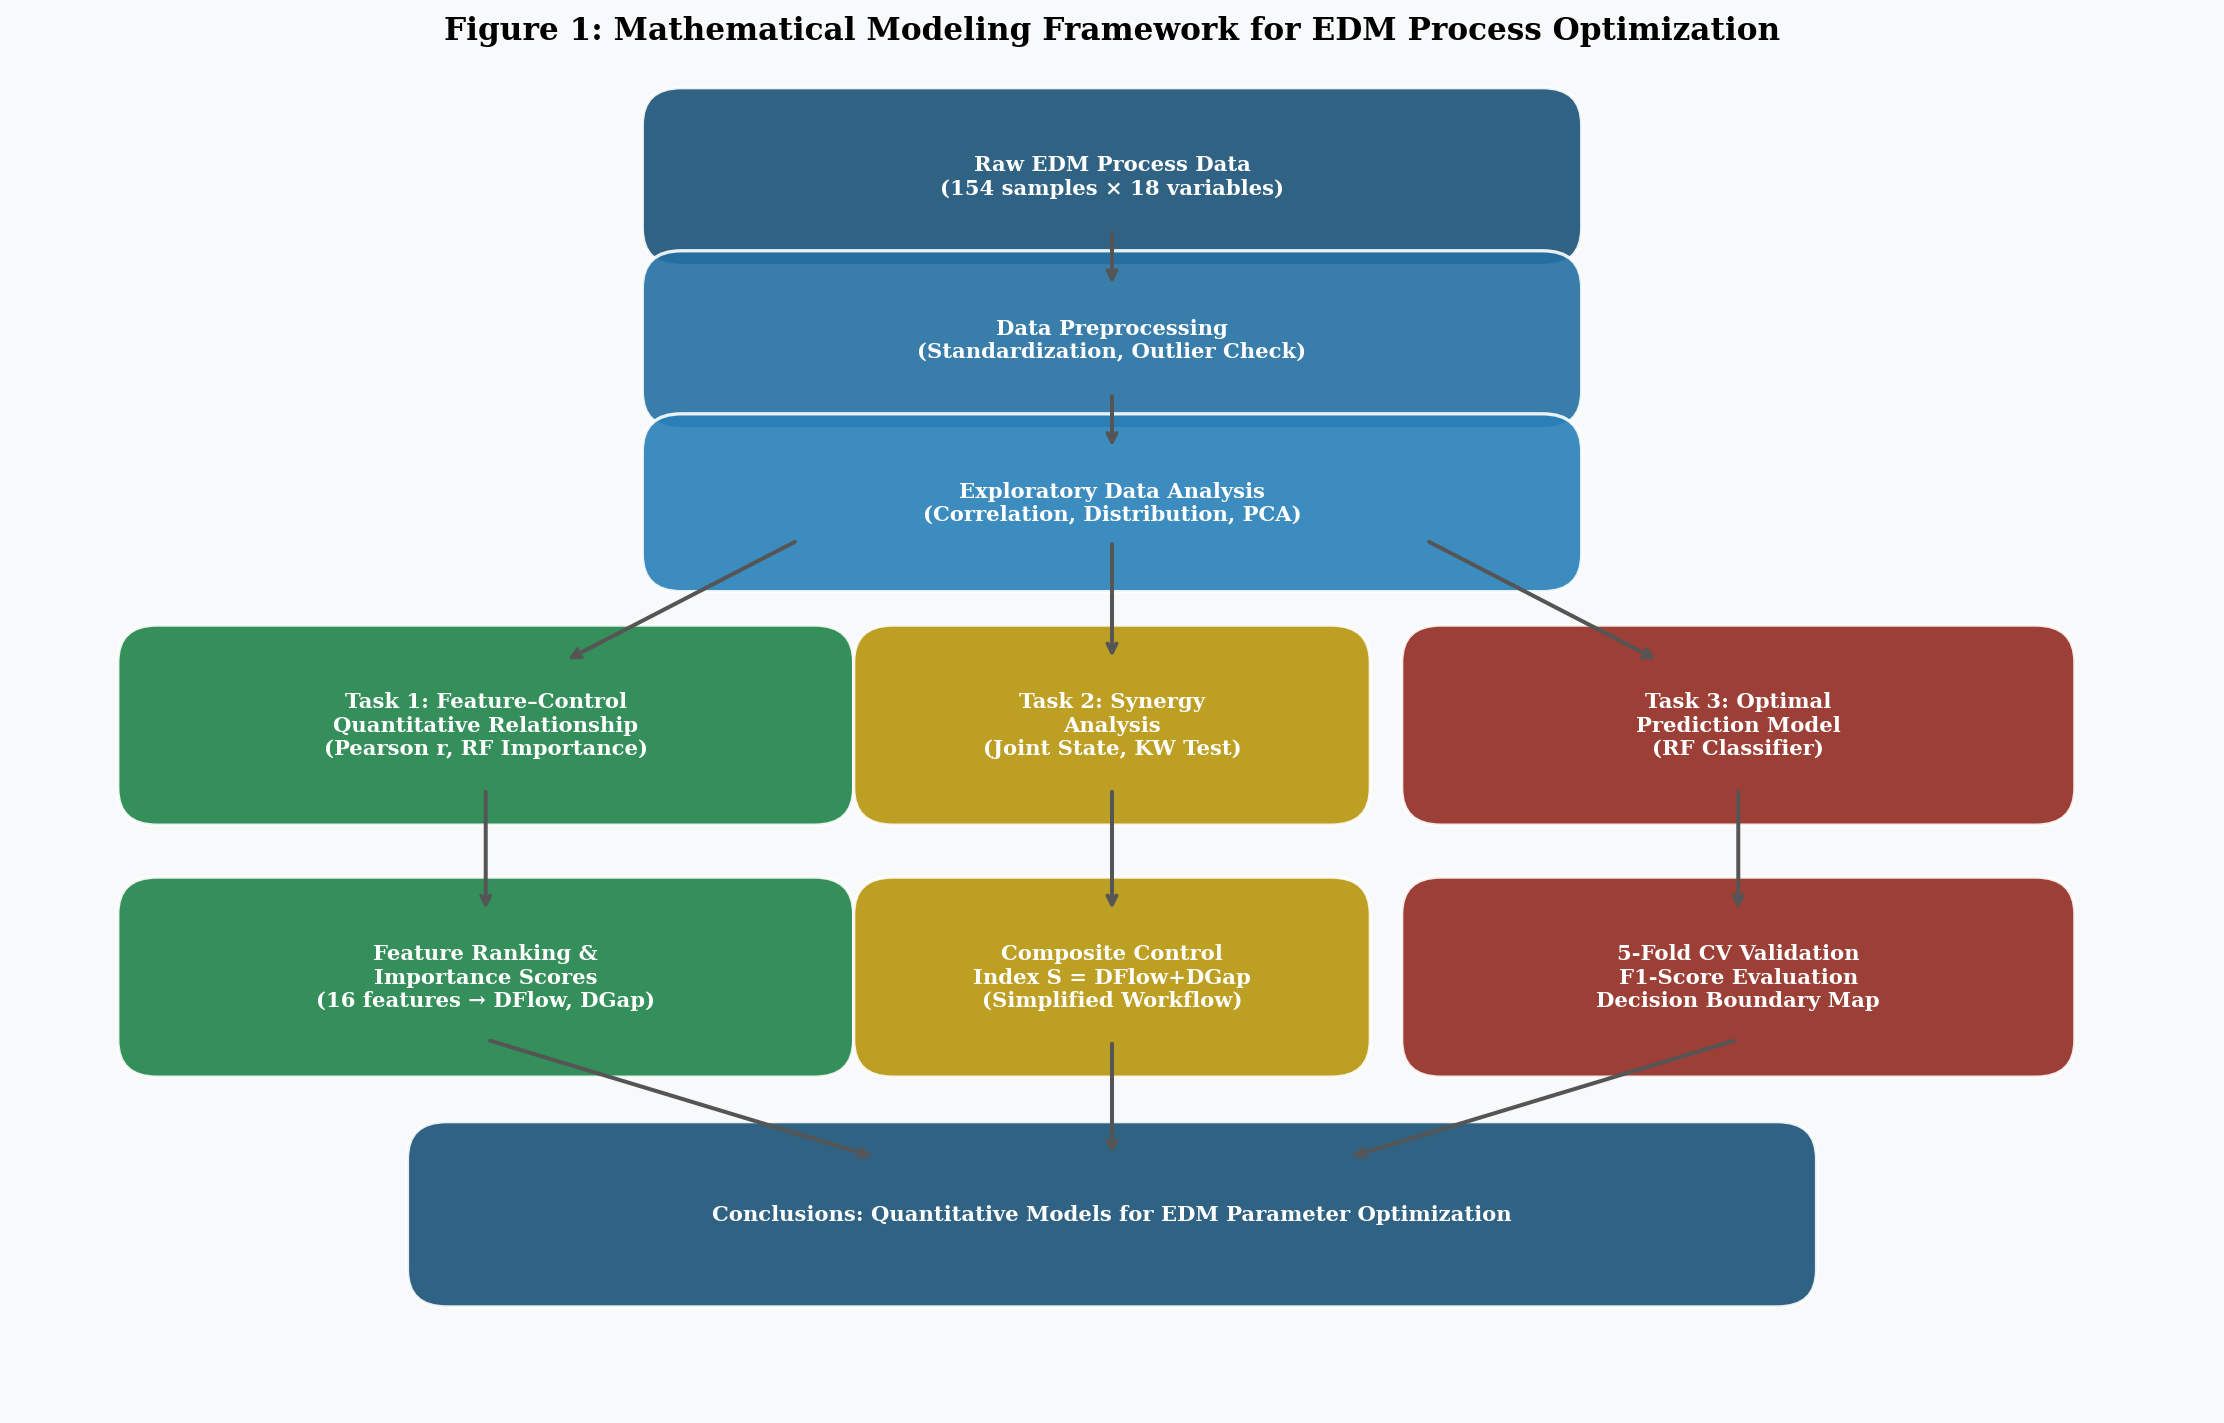
\includegraphics[width=0.88\textwidth]{outputs/Fig12_Flowchart.png}
\caption{总体建模技术路线图。图中从原始数据出发，经数据预处理与探索性分析后，分三条并行支路分别解决问题一（特征关系量化）、问题二（协同调控）和问题三（预测模型），最终汇总于结论。}
\label{fig:flowchart}
\end{figure}

如图\ref{fig:flowchart}所示，问题一的核心工作是建立脉冲特征与控制变量之间的定量映射，采用线性统计方法（Pearson相关）和非线性评估方法（随机森林特征重要性）双线索并行；问题二的核心是揭示DFlow与DGap的联合统计规律并构造可操作的协同调控指标；问题三则通过多模型比较与交叉验证确定最优预测模型组合。三个问题之间具有递进性：问题一的特征重要性排序为问题三的建模奠定特征选择基础，问题二的联合状态分析则为问题三的模型结构选择提供先验依据。

\section{符号说明}

本文涉及的主要数学符号与统计量定义见表\ref{tab:symbols}。

\begin{table}[H]
\centering
\caption{主要符号及说明}
\label{tab:symbols}
\begin{tabular}{>{\centering\arraybackslash}p{4.5cm}p{9.5cm}}
\toprule
符号 & 含义 \\
\midrule
$n=154$ & 样本总数 \\
$p=16$ & 脉冲特征维数 \\
$X=(x_1,x_2,\ldots,x_{16})\in\mathbb{R}^{p}$ & 16维脉冲特征向量 \\
$y_f\in\{-1,0,+1\}$ & 工作液流量控制变量（DFlow） \\
$y_g\in\{-1,0,+1\}$ & 放电间隙控制变量（DGap） \\
$r_{x_j,y}$ & 第$j$个特征与控制变量$y$之间的Pearson相关系数 \\
$I_j^{(f)},I_j^{(g)}$ & 特征$x_j$对DFlow、DGap的随机森林重要性 \\
$S=y_f+y_g$ & 复合控制指标，取值为$\{-2,-1,0,1,2\}$ \\
$H$ & Kruskal--Wallis检验统计量 \\
$\chi^2$ & 卡方独立性检验统计量 \\
$P_k,R_k$ & 第$k$类的精确率（Precision）与召回率（Recall） \\
$F_1^{\text{macro}}$ & 宏平均F1分数 \\
$\hat{y}_f,\hat{y}_g$ & 模型对DFlow、DGap的预测值 \\
\bottomrule
\end{tabular}
\end{table}

\section{问题分析}

\subsection{问题的数学抽象}

从数学建模角度来看，本题的三个问题具有不同的本质特征，需要采用不同的方法论框架。

问题一属于\textbf{统计关系识别问题}。给定样本矩阵$\bm{X}\in\mathbb{R}^{n\times p}$和离散响应向量$\bm{y}_f,\bm{y}_g\in\{-1,0,+1\}^n$，目标是量化每个特征$x_j$对$y_f$或$y_g$的边际贡献与综合贡献。这里存在两个挑战：其一，$x_j$与$y$之间的关系未必是线性的，单纯依靠Pearson相关系数可能低估非线性贡献；其二，16个特征之间存在较强共线性（如BSM\_B\_MeanT与CSM\_C\_MeanT之间的相关系数高达$-0.9438$），单特征分析无法反映特征间的交互信息。因此，需要综合线性与非线性两类方法进行交叉验证。

问题二属于\textbf{联合分布与调控简化问题}。其核心是：在给定$\bm{y}_f$和$\bm{y}_g$均为离散类别变量的条件下，判断二者是否存在统计依赖关系，以及这种依赖关系能否支撑一个降维的、可操作的协同控制方案。值得注意的是，依赖关系既可以是线性的（相关），也可以是非线性的（联合分布结构），因此需同时考察相关系数检验与列联表独立性检验。

问题三属于\textbf{有监督三分类预测问题}。特别地，DFlow在三个类别上的样本分布极为不均衡（类别$-1$仅5个样本，类别$0$有128个，类别$+1$有21个），这导致常规的准确率指标失效，需引入对类别不均衡鲁棒的Macro-F1指标；同时，样本量有限（$n=154$）且特征维度相对较高（$p=16$），需注意过拟合风险，应通过交叉验证评估模型的泛化性能。

\subsection{方法选择的依据}

基于上述分析，本文按照如下逻辑选取分析方法：
\begin{enumerate}[label=(\arabic*),leftmargin=2em]
\item 用\textbf{Pearson相关分析}提供线性关系的基准度量，并通过显著性检验确认有效特征；
\item 用\textbf{随机森林特征重要性}弥补线性方法的不足，捕获非线性贡献与特征交互效应，并通过节点纯度增益提供可解释的重要性排序；
\item 用\textbf{PCA}消除共线性干扰、发现数据的主要变化方向，并通过低维散点图直观评估类别可分性；
\item 用\textbf{LDA}明确各类别在最优判别方向上的分离程度，作为特征表达能力的直接验证；
\item 用\textbf{卡方检验与Kruskal--Wallis检验}分别从列联表独立性和特征分布差异两个角度支撑协同调控的统计依据；
\item 用\textbf{5折交叉验证的Macro-F1}作为最终预测模型的选择准则，兼顾性能与泛化稳定性。
\end{enumerate}

\section{模型假设}

为保证建模的可实施性与结论的有效解释范围，本文作如下合理假设：

\begin{enumerate}[label=(\arabic*),leftmargin=2em]
\item \textbf{数据独立性假设：}154个样本来源于相同类型的加工场景，各样本之间相互独立，不存在时序依赖或批次效应；
\item \textbf{特征充分性假设：}16个脉冲特征参数已能够有效表征加工过程中的主要放电状态，测量误差相对于特征变化幅度可忽略不计；
\item \textbf{类别编码一致性假设：}DFlow与DGap的取值$\{-1,0,+1\}$分别对应"减小/低、保持/中、增大/高"三种离散控制状态，且编码方向在所有样本中保持一致；
\item \textbf{稳态加工假设：}每组样本均采集自加工状态相对稳定的时刻，不包含加工启动、停机或显著异常放电的瞬态数据；
\item \textbf{模型适用范围假设：}本文所建模型适用于与数据来源相同或相近的加工工况，不直接外推至材料、电极类型或加工参数差异显著的工况。
\end{enumerate}

\section{数据预处理与探索性分析}

\subsection{数据集结构与类别分布}

数据集共包含154个样本和18个字段，其中16个为脉冲特征输入变量，2个为离散控制变量输出。16个特征按放电脉冲类型（A、B、C、I四类）和特征属性（均值时间特征、标准差时间特征、负载均值特征、负载标准差特征）组织，形成$4\times4=16$个维度的特征矩阵。

两个控制变量的类别分布情况见表\ref{tab:distribution}。

\begin{table}[H]
\centering
\caption{数据集两个控制变量的类别分布统计}
\label{tab:distribution}
\begin{tabular}{ccccccc}
\toprule
变量 & 物理意义 & 类别$-1$ & 类别$0$ & 类别$+1$ & 总样本数 & 分布特征 \\
\midrule
DFlow & 工作液流量 & 5（3.2\%） & 128（83.1\%） & 21（13.6\%） & 154 & 极度不均衡 \\
DGap  & 放电间隙 & 33（21.4\%） & 86（55.8\%） & 35（22.7\%） & 154 & 相对均衡 \\
\bottomrule
\end{tabular}
\end{table}

由表\ref{tab:distribution}可以发现两个重要规律：第一，DFlow在类别$0$上的占比高达83.1\%，意味着在当前数据对应的加工条件下，绝大多数时刻系统工作液流量处于中性状态，极少数样本属于流量增大（13.6\%）或减小（3.2\%）的状态，这种严重的类别不均衡将直接影响后续分类模型的训练与评估策略；第二，DGap的分布较为均衡，三类样本数量相差不超过三倍，表明在数据采集的实验工况下，放电间隙的调节行为更为活跃多样。

上述分布差异也在一定程度上反映了两个控制变量的物理特性：放电间隙通常需要根据极间状态频繁、精细地调整，而工作液流量的调节更多依赖宏观工况判断，单次调节后往往维持较长时间，因此中性状态的占比更高。这一物理解释支持了数据分布的合理性，同时也说明对两个变量应采用不同评估体系。

\subsection{脉冲特征描述性统计}

16个脉冲特征的完整描述性统计结果见表\ref{tab:descriptive}。

\begin{table}[H]
\centering
\caption{16个脉冲特征的描述性统计}
\label{tab:descriptive}
\begin{tabular}{ccccc}
\toprule
特征名称 & 均值 & 标准差 & 最小值 & 最大值 \\
\midrule
ASM\_A\_MeanT & $-4.656$ & $0.111$ & $-4.960$ & $-4.380$ \\
ASD\_A\_SDevT & $0.070$ & $0.066$ & $0.000$ & $0.390$ \\
BSM\_B\_MeanT & $0.816$ & $0.328$ & $0.040$ & $1.140$ \\
BSD\_B\_SDevT & $0.115$ & $0.112$ & $0.000$ & $0.450$ \\
CSM\_C\_MeanT & $5.462$ & $0.313$ & $5.100$ & $6.100$ \\
CSD\_C\_SDevT & $0.108$ & $0.101$ & $0.000$ & $0.380$ \\
ISM\_I\_MeanT & $2.188$ & $0.546$ & $0.810$ & $2.910$ \\
ISD\_I\_SDevT & $0.230$ & $0.188$ & $0.000$ & $0.770$ \\
ALM\_A\_MeanT & $-4.653$ & $0.077$ & $-4.850$ & $-4.500$ \\
ALD\_A\_SDevT & $0.097$ & $0.054$ & $0.010$ & $0.260$ \\
BLM\_B\_MeanT & $0.843$ & $0.258$ & $0.270$ & $1.140$ \\
BLD\_B\_SDevT & $0.199$ & $0.133$ & $0.000$ & $0.470$ \\
CLM\_C\_MeanT & $5.454$ & $0.258$ & $5.120$ & $5.870$ \\
CLD\_C\_SDevT & $0.188$ & $0.110$ & $0.000$ & $0.370$ \\
ILM\_I\_MeanT & $2.260$ & $0.394$ & $1.070$ & $2.790$ \\
ILD\_I\_SDevT & $0.396$ & $0.211$ & $0.030$ & $0.940$ \\
\bottomrule
\end{tabular}
\end{table}

从表\ref{tab:descriptive}可以归纳出若干规律性特征。首先，ASM\_A\_MeanT（均值约$-4.656$）与ALM\_A\_MeanT（均值约$-4.653$）的数值分布高度相似，标准差分别仅为$0.111$和$0.077$，说明A类脉冲的时间特征与负载时间特征在整体尺度上接近且波动较小，反映了A类放电脉冲时间较为稳定。其次，BSM\_B\_MeanT与BLM\_B\_MeanT（均值分别为$0.816$和$0.843$）、CSM\_C\_MeanT与CLM\_C\_MeanT（均值分别为$5.462$和$5.454$）均表现出相近的均值，但标准差明显较大，说明B类和C类脉冲特征在不同加工状态下具有更大的变异范围。此外，标准差类特征（如BSD、CSD、ILD等）普遍存在较大的变异系数，暗示放电过程的时间波动性在不同状态下差异显著，这类特征可能对控制变量具有较强的区分能力。

\subsection{数据整体分布的可视化分析}

图\ref{fig:data_overview}从类别分布饼图、DFlow--DGap联合频次热图以及各特征分DGap类别的小提琴图三个维度，对数据集进行了全面的可视化呈现。

\begin{figure}[H]
\centering
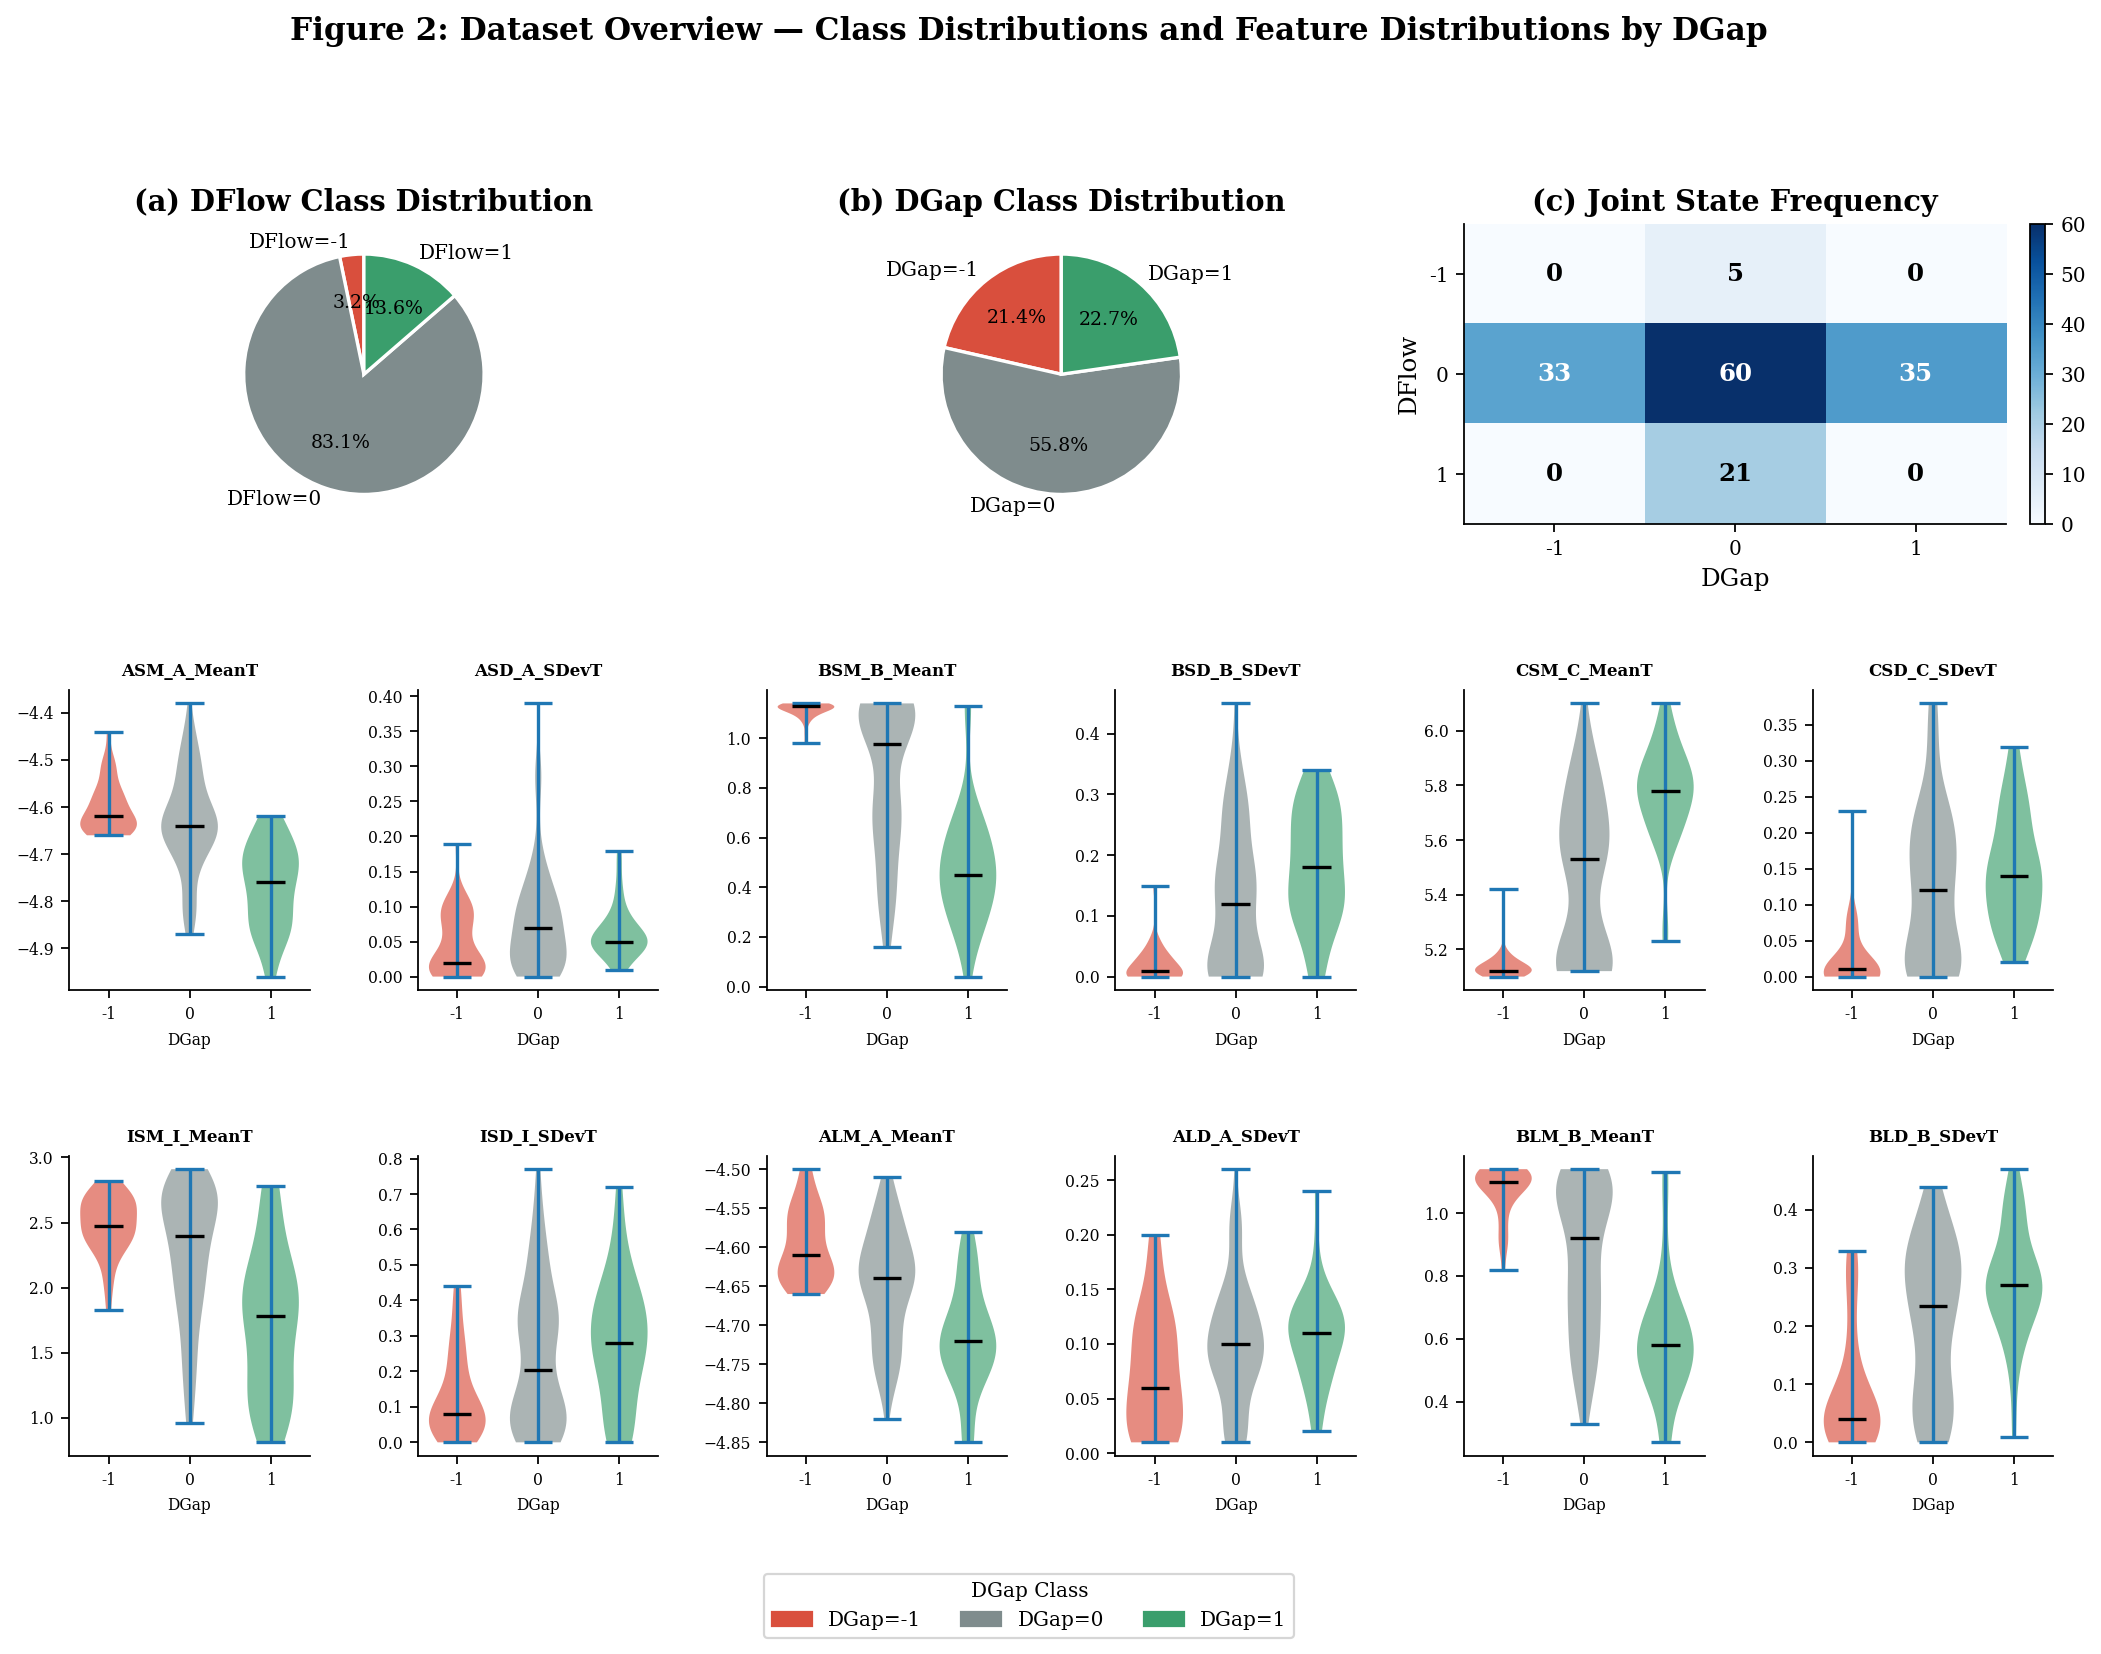
\includegraphics[width=\textwidth]{outputs/Fig1_Data_Overview.png}
\caption{数据集总体分布与特征分布可视化。图(a)与图(b)分别展示DFlow和DGap的类别分布饼图；图(c)给出DFlow--DGap联合频次热图；图(d)至图(s)为16个特征按DGap三类分组的小提琴图，红色、灰色、绿色分别对应$DGap=-1,0,+1$三类。}
\label{fig:data_overview}
\end{figure}

从图\ref{fig:data_overview}的小提琴图中可以直观观察到：CSM\_C\_MeanT、BSM\_B\_MeanT、CLM\_C\_MeanT、BLM\_B\_MeanT等特征在三类DGap状态下的分布差异最为显著，三条小提琴图的形态和中位数位置均存在明显偏移，说明这些特征具有较强的DGap区分能力；而ASD\_A\_SDevT等特征在三类状态下的分布几乎完全重叠，说明其对DGap的判别贡献有限。这些初步观察与后续定量分析的结论保持一致，为后续特征重要性评估提供了直观的先验支撑。

联合频次热图（图(c)）进一步表明，DFlow类别$0$与DGap所有类别的组合在频次上均远高于DFlow类别$\pm1$的情形，其中$(DFlow=0,DGap=0)$组合出现频次最高，达60次。这一不均衡的联合分布揭示了数据采集工况的内在规律，也是后续协同调控分析的关键起点。

在数据标准化处理上，所有特征均进行$z$-score标准化：
\begin{equation}
\tilde{x}_{ij}=\frac{x_{ij}-\bar{x}_j}{s_j},
\end{equation}
其中$\bar{x}_j$为第$j$个特征的样本均值，$s_j$为其样本标准差。标准化消除了不同特征量纲差异的影响，保证后续PCA、LDA和分类模型的计算结果不受特征尺度干扰。

\section{问题一：脉冲特征与控制变量的量化关系分析}

\subsection{Pearson线性相关分析}

\subsubsection{模型建立}

Pearson相关系数是衡量两个随机变量之间线性相关程度的经典统计量。对于第$j$个脉冲特征$x_j$与控制变量$y$（DFlow或DGap），其Pearson相关系数定义为：
\begin{equation}
r_{x_j,y}=\frac{\displaystyle\sum_{i=1}^{n}(x_{ij}-\bar{x}_j)(y_i-\bar{y})}{\displaystyle\sqrt{\sum_{i=1}^{n}(x_{ij}-\bar{x}_j)^2}\cdot\sqrt{\sum_{i=1}^{n}(y_i-\bar{y})^2}},
\label{eq:pearson}
\end{equation}
其中$\bar{x}_j$与$\bar{y}$分别为对应变量的样本均值，$r_{x_j,y}\in[-1,1]$。当$|r|$趋近于1时，表示两变量之间存在强线性相关；$|r|$趋近于0时，表示线性关系微弱。为判断相关系数的统计显著性，构造$t$统计量：
\begin{equation}
t=\frac{r\sqrt{n-2}}{\sqrt{1-r^2}}\sim t(n-2),
\end{equation}
在显著性水平$\alpha=0.05$下对所有特征进行双侧检验。

\subsubsection{分析结果}

全部16个特征与两个控制变量的完整Pearson相关系数见表\ref{tab:corr-full}。

\begin{table}[H]
\centering
\caption{16个脉冲特征与DFlow、DGap的Pearson相关系数}
\label{tab:corr-full}
\begin{tabular}{ccc}
\toprule
特征名称 & $r$（DFlow） & $r$（DGap） \\
\midrule
ASM\_A\_MeanT & $-0.0541$ & $-0.5068^{***}$ \\
ASD\_A\_SDevT & $0.4234^{***}$ & $0.0733$ \\
BSM\_B\_MeanT & $-0.2592^{**}$ & $-0.6434^{***}$ \\
BSD\_B\_SDevT & $0.4640^{***}$ & $0.4723^{***}$ \\
CSM\_C\_MeanT & $0.3066^{***}$ & $0.6693^{***}$ \\
CSD\_C\_SDevT & $0.4388^{***}$ & $0.4073^{***}$ \\
ISM\_I\_MeanT & $0.0326$ & $-0.4624^{***}$ \\
ISD\_I\_SDevT & $0.3266^{***}$ & $0.2750^{***}$ \\
ALM\_A\_MeanT & $-0.2391^{**}$ & $-0.5202^{***}$ \\
ALD\_A\_SDevT & $0.2319^{**}$ & $0.1906^{*}$ \\
BLM\_B\_MeanT & $-0.3751^{***}$ & $-0.6200^{***}$ \\
BLD\_B\_SDevT & $0.3265^{***}$ & $0.4626^{***}$ \\
CLM\_C\_MeanT & $0.4508^{***}$ & $0.6302^{***}$ \\
CLD\_C\_SDevT & $0.3102^{***}$ & $0.4000^{***}$ \\
ILM\_I\_MeanT & $-0.1906^{*}$ & $-0.4042^{***}$ \\
ILD\_I\_SDevT & $0.1707^{*}$ & $0.4276^{***}$ \\
\bottomrule
\multicolumn{3}{l}{\footnotesize 注：$^{*}p<0.05$，$^{**}p<0.01$，$^{***}p<0.001$}
\end{tabular}
\end{table}

\subsubsection{结果解释}

由表\ref{tab:corr-full}可归纳以下关键规律：

\textbf{（1）DGap的相关特征更为突出。}DGap与CSM\_C\_MeanT（$r=0.6693$）、BSM\_B\_MeanT（$r=-0.6434$）、CLM\_C\_MeanT（$r=0.6302$）的相关系数绝对值均超过0.63，远高于DFlow对应的最大值（0.4640），表明DGap的变化在脉冲特征空间中具有更强的线性可辨性。

\textbf{（2）DFlow的相关特征以标准差类为主。}与DFlow相关性最强的三个特征——BSD\_B\_SDevT（$r=0.4640$）、CLM\_C\_MeanT（$r=0.4508$）、CSD\_C\_SDevT（$r=0.4388$）中，有两个为标准差类特征，说明DFlow的变化主要体现在放电时间波动性上，而非均值水平。这在物理上是合理的：工作液流量的变化首先影响极间介质对流、改变放电稳定性，进而导致脉冲时间标准差增大或减小，而对各类脉冲的均值时间影响相对间接。

\textbf{（3）C类特征是两个控制变量的共同敏感区域。}CLM\_C\_MeanT对DFlow（$r=0.4508$）和DGap（$r=0.6302$）均具有较高相关性，CSM\_C\_MeanT对DGap的相关性最强（$r=0.6693$），说明C类脉冲的时间特征是综合反映加工状态的核心指标，其变化能同时表征两个控制变量的调节方向。

图\ref{fig:corr}从特征间相关矩阵（左图）和特征与控制变量相关系数条形图（右图）两个维度进一步呈现了相关分析结果。

\begin{figure}[H]
\centering
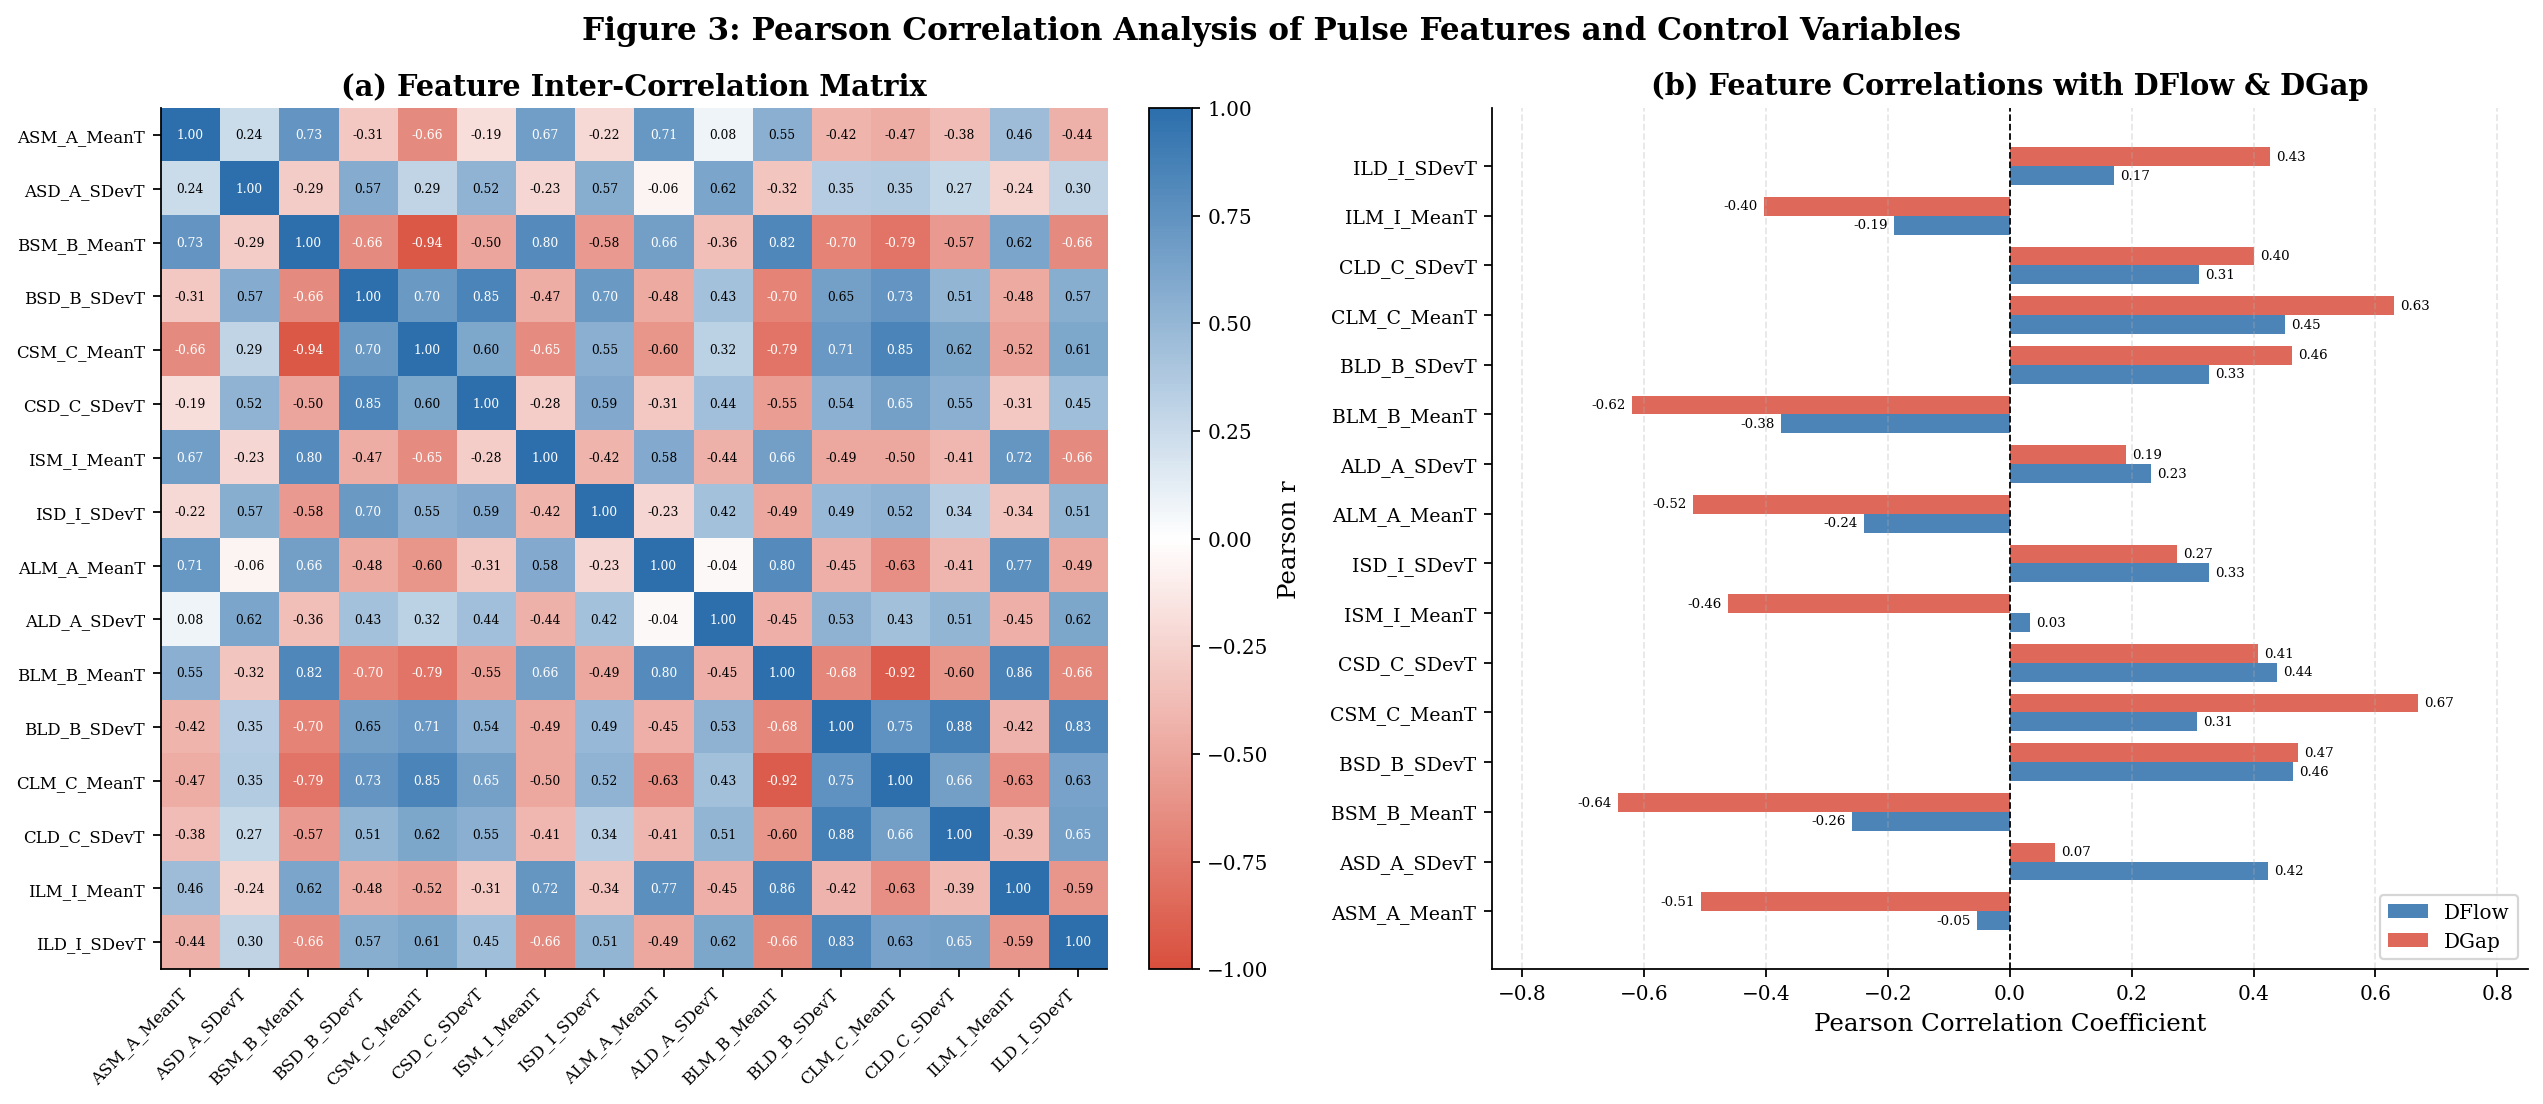
\includegraphics[width=\textwidth]{outputs/Fig2_Correlation_Analysis.png}
\caption{脉冲特征相关分析结果。左图为16个脉冲特征之间的Pearson相关矩阵热图，颜色深浅表示相关系数绝对值大小，红色为负相关，蓝色为正相关；右图为各特征与DFlow（蓝色）、DGap（红色）的Pearson相关系数水平条形图，正负方向分别对应正相关与负相关。}
\label{fig:corr}
\end{figure}

从图\ref{fig:corr}左图可以清晰看出，特征矩阵中存在多个高度相关的特征对。其中，BSM\_B\_MeanT与CSM\_C\_MeanT之间的相关系数高达$-0.9438$，BLM\_B\_MeanT与CLM\_C\_MeanT之间达$-0.9162$，BSM\_B\_MeanT与BLM\_B\_MeanT之间达$0.8228$；此外还存在BSD\_B\_SDevT—CSD\_C\_SDevT（$r=0.8478$）、BLD\_B\_SDevT—CLD\_C\_SDevT（$r=0.8758$）、BLM\_B\_MeanT—ILM\_I\_MeanT（$r=0.8597$）等共9对强相关特征对（$|r|>0.8$）。这种高度共线性的存在说明16个特征并非相互独立，其中蕴含大量冗余信息，若不进行合理的降维或特征选择，在建立分类模型时可能引起参数估计不稳定的问题。

从图\ref{fig:corr}右图可以进一步确认：BSM\_B\_MeanT和BLM\_B\_MeanT对DGap均呈显著负相关，CSM\_C\_MeanT和CLM\_C\_MeanT均呈显著正相关，而这两对特征之间本身高度负相关——这一现象在物理上可以理解为：B类脉冲的时间增长与C类脉冲的时间缩短往往同时发生，反映了放电过程中不同能量级别脉冲之间的此消彼长关系。

\subsection{特征间相关结构的层次聚类分析}

为进一步揭示16个脉冲特征之间的内在聚类结构，以相关距离$d_{jk}=1-|r_{jk}|$为相异度量，采用平均链接法（Average Linkage）对特征进行层次聚类，结果如图\ref{fig:dendrogram}所示。

\begin{figure}[H]
\centering
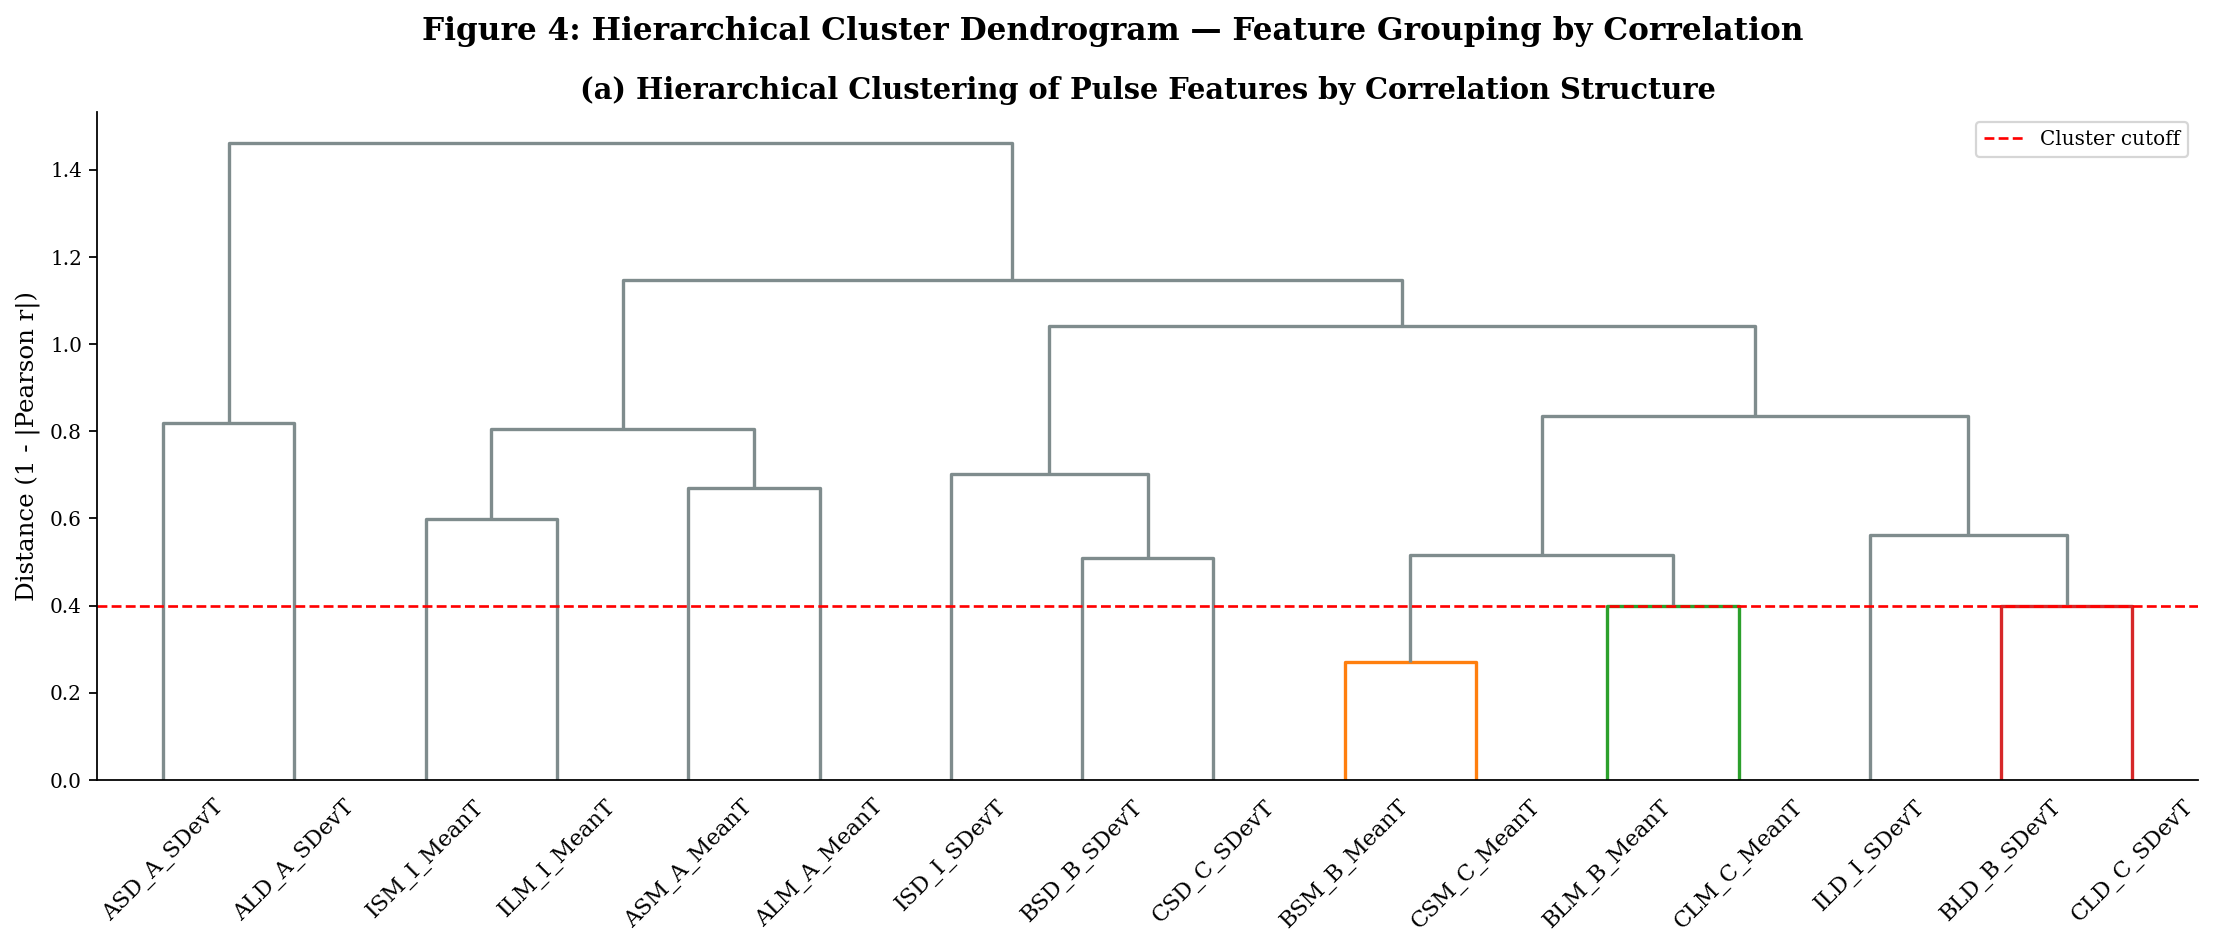
\includegraphics[width=\textwidth]{outputs/Fig11_Dendrogram.png}
\caption{16个脉冲特征按相关结构的层次聚类树状图。纵轴为相关距离$d=1-|r|$，切割阈值设为0.4（红色虚线），该阈值对应$|r|>0.6$的强相关组。聚类树揭示了特征群的内在结构，相同聚类的特征对控制变量的贡献方向相近，可作为特征选择或降维的参考依据。}
\label{fig:dendrogram}
\end{figure}

从图\ref{fig:dendrogram}中可见，在切割阈值$d=0.4$（对应$|r|>0.6$）处，16个特征大致分为三个主要聚类群：第一群以B类与C类脉冲的均值时间特征为核心（BSM\_B\_MeanT、CSM\_C\_MeanT、BLM\_B\_MeanT、CLM\_C\_MeanT、ISM\_I\_MeanT、ILM\_I\_MeanT），这些特征之间相关性极强，且对DGap的影响最为显著；第二群以B、C类脉冲的标准差特征为主（BSD\_B\_SDevT、CSD\_C\_SDevT、BLD\_B\_SDevT、CLD\_C\_SDevT、ILD\_I\_SDevT等），这些特征主要反映放电时间的稳定性，与DFlow的相关性相对较强；第三群以A类脉冲特征为主（ASM\_A\_MeanT、ALM\_A\_MeanT、ASD\_A\_SDevT、ALD\_A\_SDevT），该类特征相互独立性较高，且在整体上对控制变量的影响中等。

这一聚类结果与物理意义高度吻合。A、B、C、I四类脉冲在EDM过程中分别对应不同的放电能量等级与放电模式：A类通常代表短路脉冲，其时间特征受加工状态扰动较小；B类和C类分别代表正常放电与弧放电，其时间比例随间隙状态和流量变化而显著变化。因此聚类结果为后续特征工程提供了有意义的物理分组依据。

\subsection{随机森林特征重要性评估}

\subsubsection{模型建立}

为弥补Pearson相关分析仅能刻画线性关系的局限，本文引入随机森林（Random Forest，RF）模型，以基于不纯度减少（Impurity Decrease）的特征重要性量化各特征对分类结果的综合贡献。

随机森林由$T$棵决策树组成，第$t$棵树通过对原始样本的有放回自助抽样（Bootstrap）构建。第$j$个特征的重要性定义为：
\begin{equation}
I_j=\frac{1}{T}\sum_{t=1}^{T}\sum_{v\in\mathcal{V}_t(j)}\frac{n_v}{n}\cdot\Delta G(v),
\label{eq:rf_importance}
\end{equation}
其中$\mathcal{V}_t(j)$为第$t$棵树中所有以特征$j$作为分裂变量的内部节点集合，$n_v$为到达节点$v$的样本数，$n$为总样本数，$\Delta G(v)$为节点$v$分裂前后的基尼不纯度（Gini Impurity）之差：
\begin{equation}
\Delta G(v)=G(v)-\frac{n_{v_L}}{n_v}G(v_L)-\frac{n_{v_R}}{n_v}G(v_R),
\end{equation}
其中$G(v)=1-\sum_{k}p_{vk}^2$为节点$v$的基尼不纯度，$p_{vk}$为节点$v$中第$k$类的样本比例，$v_L$和$v_R$分别为$v$的左右子节点。最终将各特征的重要性归一化，使所有特征重要性之和为100\%。

在实现上，分别为DFlow和DGap训练两个独立的随机森林分类器，均设定$T=200$棵树、采用类别加权（class\_weight=`balanced'）以缓解类别不均衡问题，并对全量154个样本进行训练以获得最稳定的特征重要性估计。

\subsubsection{分析结果}

全部16个特征的重要性排序结果见表\ref{tab:rf-full}。

\begin{table}[H]
\centering
\caption{随机森林特征重要性完整排序（$n=200$棵树，全量样本训练）}
\label{tab:rf-full}
\begin{tabular}{cccccc}
\toprule
\multicolumn{3}{c}{DFlow预测模型} & \multicolumn{3}{c}{DGap预测模型} \\
\cmidrule(r){1-3}\cmidrule(l){4-6}
排名 & 特征名称 & 重要性（\%） & 排名 & 特征名称 & 重要性（\%） \\
\midrule
1  & ASM\_A\_MeanT & 13.67 & 1  & CSM\_C\_MeanT & 14.91 \\
2  & ALM\_A\_MeanT & 13.09 & 2  & BSM\_B\_MeanT & 11.25 \\
3  & CLM\_C\_MeanT & 10.96 & 3  & ILD\_I\_SDevT & 8.82 \\
4  & ASD\_A\_SDevT & 6.70  & 4  & BLM\_B\_MeanT & 7.91 \\
5  & BSM\_B\_MeanT & 6.51  & 5  & CLM\_C\_MeanT & 7.37 \\
6  & CSD\_C\_SDevT & 6.43  & 6  & ASM\_A\_MeanT & 6.86 \\
7  & CSM\_C\_MeanT & 6.08  & 7  & ILM\_I\_MeanT & 5.13 \\
8  & BSD\_B\_SDevT & 5.78  & 8  & BSD\_B\_SDevT & 5.05 \\
9  & ISM\_I\_MeanT & 5.55  & 9  & ASD\_A\_SDevT & 4.93 \\
10 & CLD\_C\_SDevT & 5.02  & 10 & ISM\_I\_MeanT & 4.79 \\
11 & BLM\_B\_MeanT & 4.93  & 11 & ALM\_A\_MeanT & 4.64 \\
12 & ISD\_I\_SDevT & 4.83  & 12 & CSD\_C\_SDevT & 4.23 \\
13 & ALD\_A\_SDevT & 3.76  & 13 & CLD\_C\_SDevT & 3.96 \\
14 & ILD\_I\_SDevT & 2.94  & 14 & ISD\_I\_SDevT & 3.80 \\
15 & BLD\_B\_SDevT & 2.65  & 15 & BLD\_B\_SDevT & 3.54 \\
16 & ILM\_I\_MeanT & 1.11  & 16 & ALD\_A\_SDevT & 2.81 \\
\bottomrule
\end{tabular}
\end{table}

图\ref{fig:importance}通过水平条形图直观呈现了特征重要性分布，并以中位数为界将特征分为高于中位数（深色）和低于中位数（浅色）两档。

\begin{figure}[H]
\centering
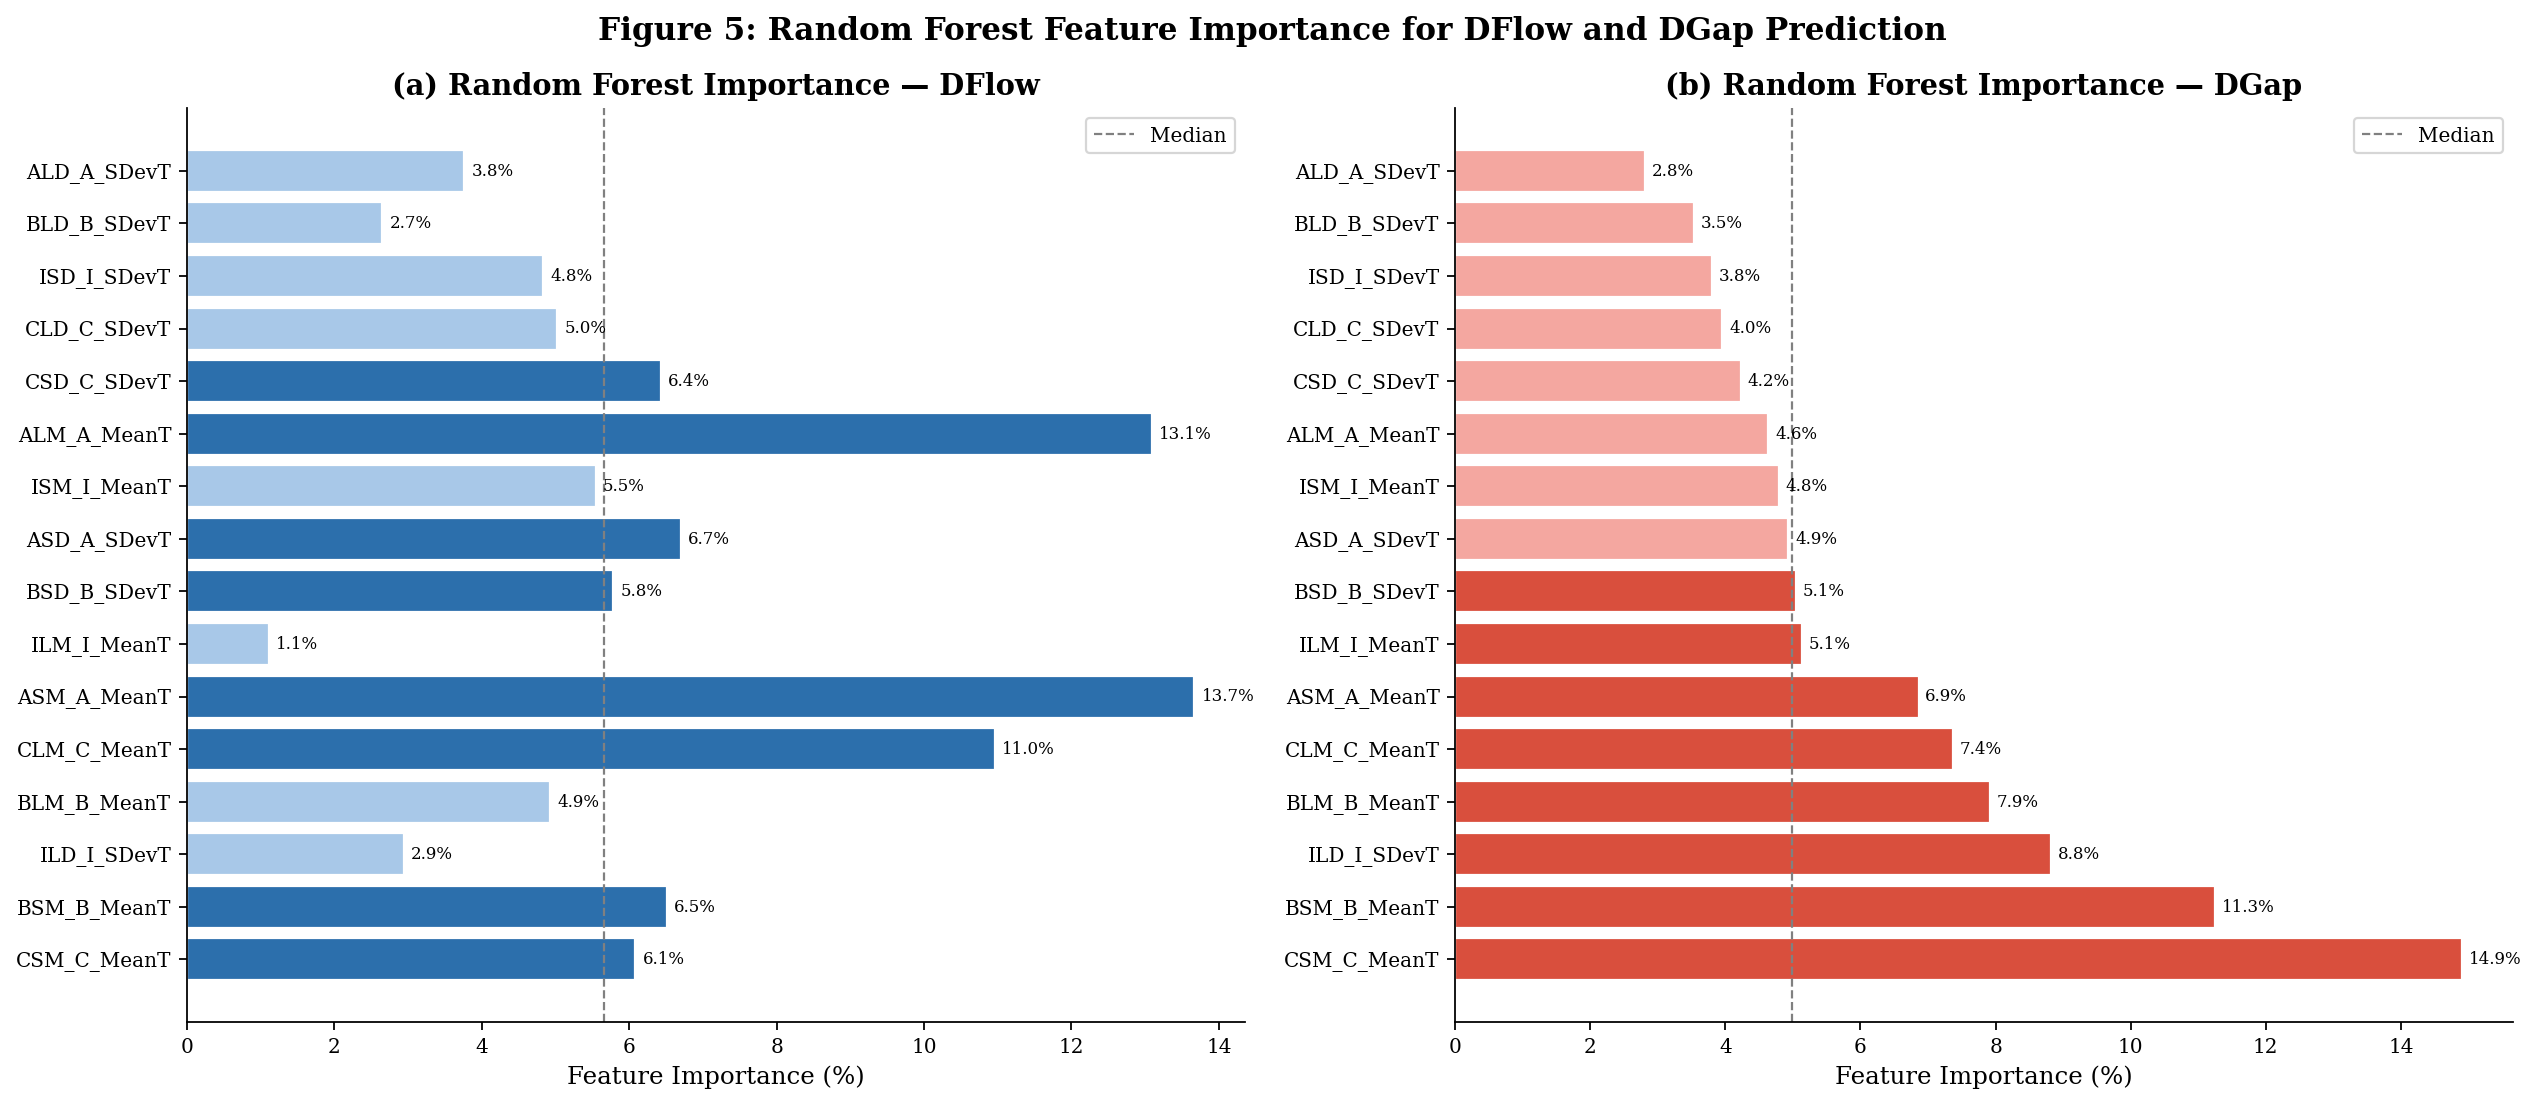
\includegraphics[width=\textwidth]{outputs/Fig4_Feature_Importance.png}
\caption{随机森林特征重要性排序条形图。左图为DFlow模型，右图为DGap模型；深色条形表示重要性高于中位数的特征，浅色条形为低于中位数的特征；虚线为中位数参考线。两图的特征排列顺序一致，均按DGap模型的重要性从大到小排序，便于对比两个模型的差异。}
\label{fig:importance}
\end{figure}

\subsubsection{结果解释}

综合表\ref{tab:rf-full}与图\ref{fig:importance}，可以得到以下重要结论：

\textbf{（1）两个模型的核心特征存在差异。}DFlow模型的最重要特征为ASM\_A\_MeanT（13.67\%）和ALM\_A\_MeanT（13.09\%），两者合计占比超过26\%，说明A类脉冲的均值时间信息对工作液流量的判别贡献最大。这与Pearson分析存在差异（A类特征对DFlow的线性相关性并不突出），反映了A类特征与DFlow之间存在非线性关联，随机森林的树结构能够捕获这种非线性信息，而Pearson系数则无法体现。DGap模型的最重要特征为CSM\_C\_MeanT（14.91\%）和BSM\_B\_MeanT（11.25\%），与Pearson分析结论一致，表明DGap的状态主要由C类和B类均值时间特征线性决定，两种方法的结论相互印证。

\textbf{（2）DGap模型的特征贡献更为集中，DFlow模型的贡献分布更为分散。}DGap模型中前3个特征合计重要性为35.0\%，而DFlow模型前3个特征合计仅为33.7\%，从整体分布来看，DGap模型的高重要性特征更集中，尾部特征的重要性下降更快。这意味着DGap的分类边界主要由少数关键特征决定，而DFlow则需要更多特征的协同表达，在建模时可能对特征的全局结构更为敏感。

\textbf{（3）ILD\_I\_SDevT是DGap模型的特殊贡献特征。}该特征在DGap模型中排名第3（8.82\%），但在Pearson相关分析中其线性相关系数仅为0.4276，排名靠后。这说明ILD\_I\_SDevT对DGap的贡献主要通过非线性交互方式实现，即它在某些特征值区间内对DGap的判别具有较强的条件区分能力，但在全局线性关系上表现并不突出。这类特征在决策树结构中往往充当"局部分裂器"，对提高整体分类精度具有不可忽视的作用。

\subsection{主成分分析（PCA）}

\subsubsection{模型建立与结果}

主成分分析（Principal Component Analysis，PCA）通过线性变换将$p$维原始特征$\bm{X}$投影到$q$维正交子空间（$q<p$），使得投影后各主成分的方差最大。PCA的数学核心是对标准化后的样本协方差矩阵$\bm{\Sigma}$进行特征分解：
\begin{equation}
\bm{\Sigma}\bm{v}_k=\lambda_k\bm{v}_k,\quad k=1,2,\ldots,p,
\end{equation}
其中$\lambda_1\geq\lambda_2\geq\cdots\geq\lambda_p\geq0$为特征值，$\bm{v}_k$为对应的特征向量（即第$k$个主成分的载荷向量），第$k$个主成分的得分向量为$\bm{z}_k=\bm{X}\bm{v}_k$。第$k$个主成分的方差贡献率为$\lambda_k/\sum_{l}\lambda_l$。

对16个标准化特征进行PCA，前6个主成分的方差贡献率及累计贡献率如表\ref{tab:pca}所示。

\begin{table}[H]
\centering
\caption{PCA前6个主成分的方差贡献率}
\label{tab:pca}
\begin{tabular}{cccc}
\toprule
主成分 & 特征值 & 方差贡献率（\%） & 累计贡献率（\%） \\
\midrule
PC1 & 9.155 & 57.22 & 57.22 \\
PC2 & 2.248 & 14.05 & 71.27 \\
PC3 & 1.086 & 6.79  & 78.07 \\
PC4 & 1.032 & 6.45  & 84.52 \\
PC5 & 0.758 & 4.74  & 89.26 \\
PC6 & 0.410 & 2.56  & 91.82 \\
\bottomrule
\end{tabular}
\end{table}

图\ref{fig:pca}给出了PCA的碎石图（Scree Plot）、基于PC1--PC2的二维散点图以及基于PC1--PC2--PC3的三维散点图，各图均按DGap类别上色。

\begin{figure}[H]
\centering
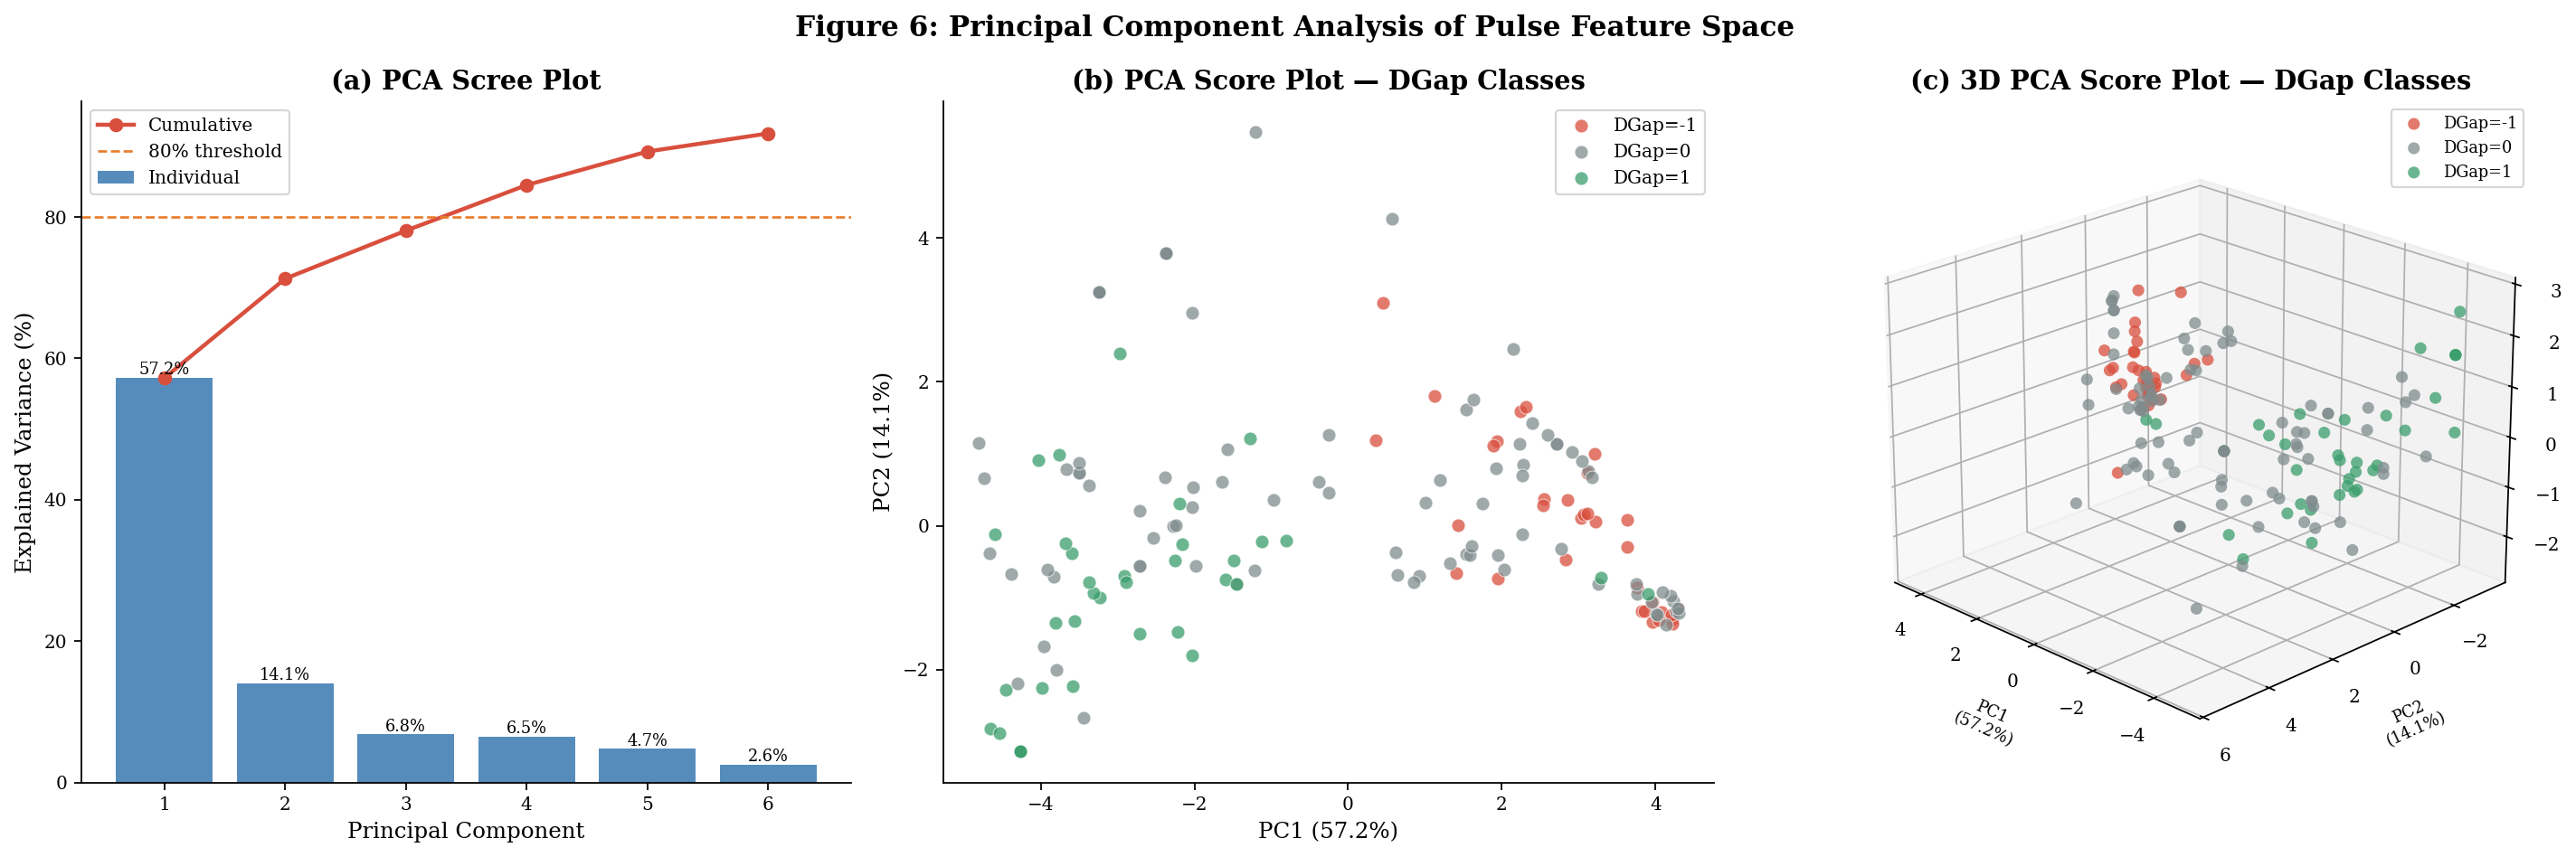
\includegraphics[width=\textwidth]{outputs/Fig3_PCA_Analysis.png}
\caption{主成分分析结果。图(a)为前6个主成分的方差贡献率碎石图，蓝色柱表示各主成分个别贡献，红色曲线为累计贡献率，橙色虚线为80\%阈值参考线；图(b)为前两个主成分（PC1--PC2）的二维得分散点图，按DGap三类着色；图(c)为前三个主成分（PC1--PC2--PC3）的三维得分散点图，同样按DGap类别着色，能够呈现更完整的类别分布结构。}
\label{fig:pca}
\end{figure}

\subsubsection{结果解释}

从表\ref{tab:pca}和图\ref{fig:pca}(a)可知，PC1单独解释了57.22\%的总方差，这一比例远高于其他主成分，说明16维特征空间中存在一个占主导地位的线性变化方向。结合载荷分析，PC1的主要载荷来自BLM\_B\_MeanT（$+0.303$）、BSM\_B\_MeanT（$+0.299$）与CLM\_C\_MeanT（$-0.295$），物理上反映了B类脉冲均值时间与C类脉冲均值时间之间的此消彼长关系；PC2的主要载荷来自ASD\_A\_SDevT（$+0.480$）、ASM\_A\_MeanT（$+0.460$）与ALD\_A\_SDevT（$+0.364$），主要反映A类脉冲时间特征的整体波动水平；PC3的主要载荷来自ALD\_A\_SDevT（$+0.521$）与CSD\_C\_SDevT（$-0.382$），反映了A类负载标准差与C类时间标准差之间的差异。

从图\ref{fig:pca}(b)的二维得分图可以看出，DGap三类样本在PC1方向上具有较好的有序分离：$DGap=-1$的样本（红色）主要分布在PC1负半轴，$DGap=+1$的样本（绿色）主要分布在PC1正半轴，$DGap=0$的样本（灰色）居中分布。这与载荷分析结论一致：PC1正方向代表B类脉冲时间增大（BSM\_B\_MeanT增大）同时C类脉冲时间减小的状态，而这种脉冲结构变化与DGap的增大方向相关。然而，三类样本在二维空间中仍存在较大重叠，说明仅靠线性降维不能完全分离三类，需引入非线性分类方法。

\subsection{线性判别分析（LDA）}

线性判别分析（Linear Discriminant Analysis，LDA）在寻求判别超平面的同时，最大化类间散度与类内散度之比：
\begin{equation}
\bm{w}^{*}=\arg\max_{\bm{w}}\frac{\bm{w}^{\top}\bm{S}_B\bm{w}}{\bm{w}^{\top}\bm{S}_W\bm{w}},
\end{equation}
其中$\bm{S}_B=\sum_{k=1}^{K}n_k(\bm{\mu}_k-\bm{\mu})(\bm{\mu}_k-\bm{\mu})^{\top}$为类间散度矩阵，$\bm{S}_W=\sum_{k=1}^{K}\sum_{i\in C_k}(\bm{x}_i-\bm{\mu}_k)(\bm{x}_i-\bm{\mu}_k)^{\top}$为类内散度矩阵，$\bm{\mu}_k$为第$k$类的样本均值，$\bm{\mu}$为总体样本均值。

LDA判别结果见图\ref{fig:lda}，各类别在LD1轴上的均值见表\ref{tab:lda}。

\begin{figure}[H]
\centering
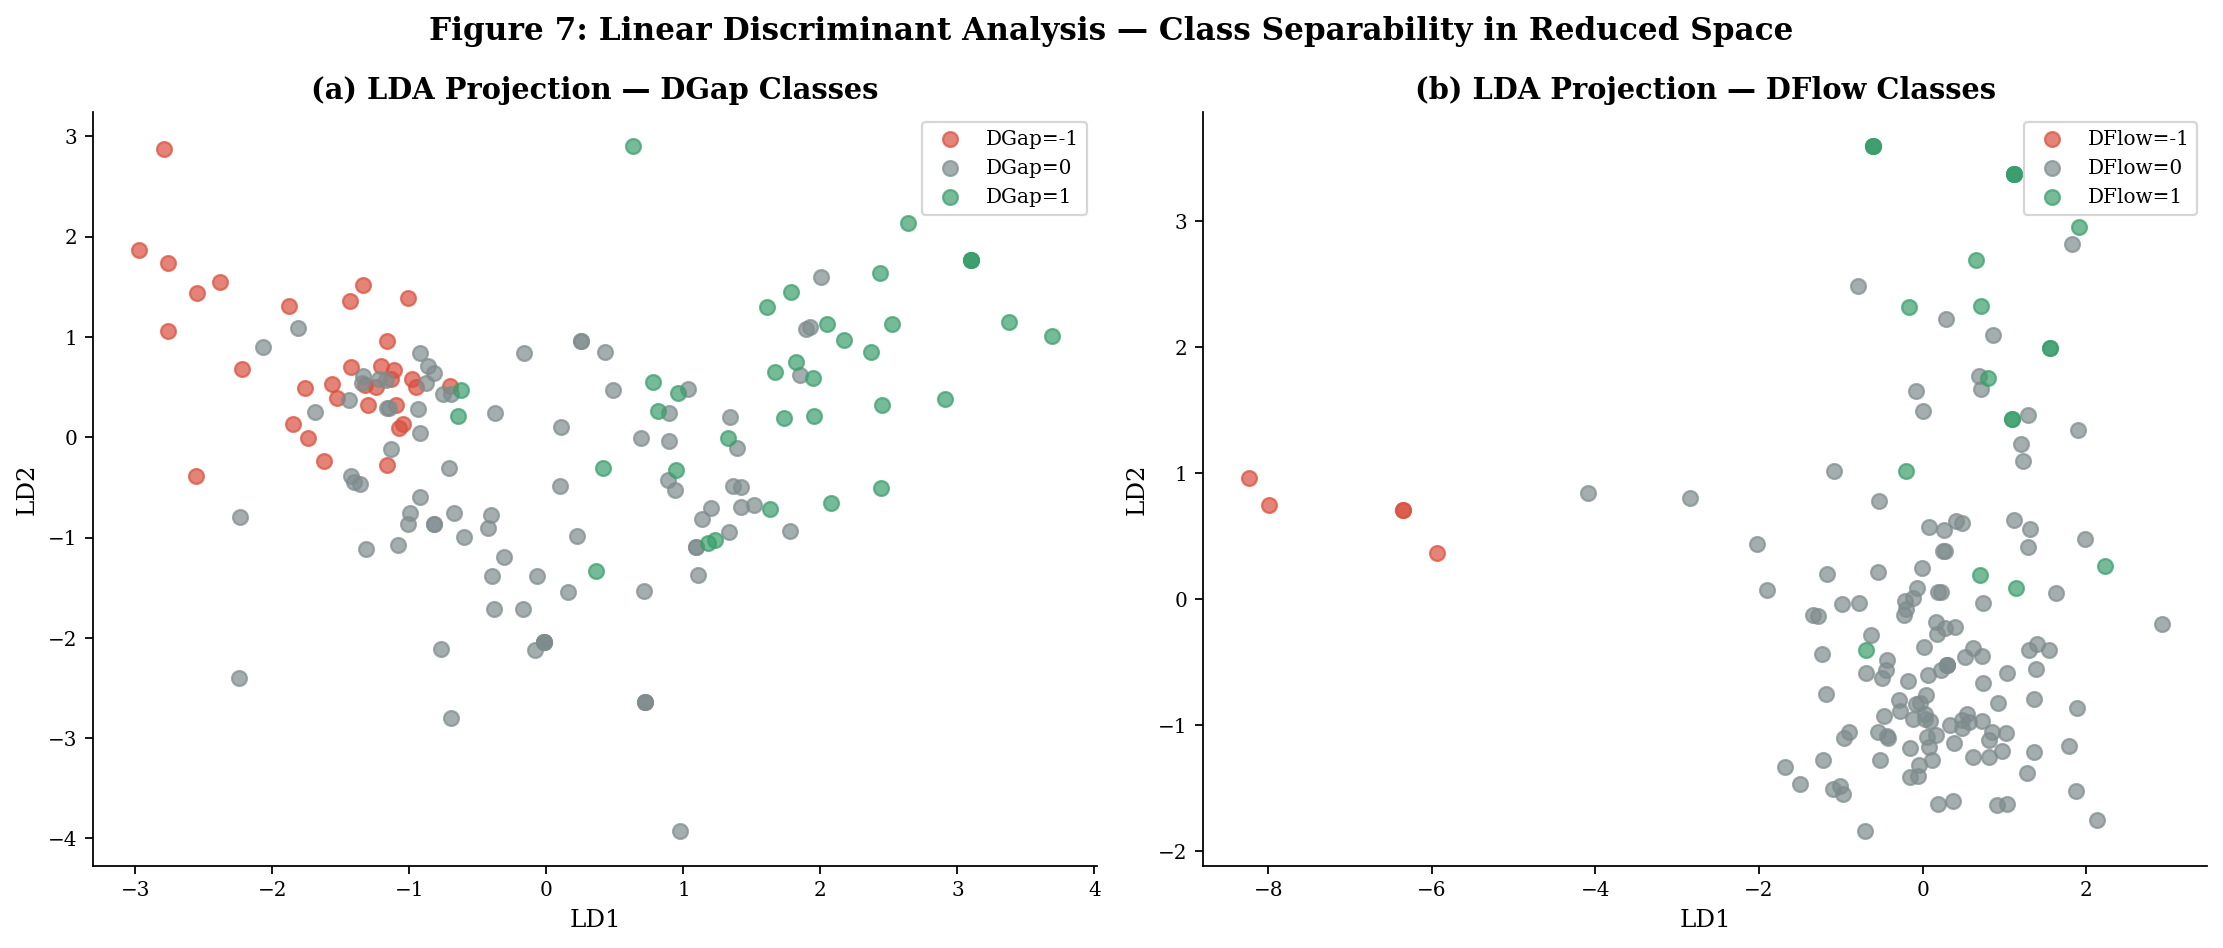
\includegraphics[width=\textwidth]{outputs/Fig6_LDA_Analysis.png}
\caption{线性判别分析结果。图(a)为DGap三类在LD1方向的密度分布直方图，图(b)为DFlow三类在LD1方向的密度分布直方图。横轴为第一判别轴LD1的投影值，纵轴为概率密度；颜色编码与图\ref{fig:data_overview}一致。LD1方向最大化类间与类内方差之比，是区分三类样本信息最丰富的线性方向。}
\label{fig:lda}
\end{figure}

\begin{table}[H]
\centering
\caption{LDA判别轴LD1上各类别的投影均值与标准差}
\label{tab:lda}
\begin{tabular}{ccccc}
\toprule
控制变量 & 类别 & LD1均值 & LD1标准差 & 类间分离程度 \\
\midrule
\multirow{3}{*}{DGap} & $-1$ & $-1.6261$ & $0.6326$ & \multirow{3}{*}{各类均值差距明显，分离良好} \\
 & $0$ & $-0.0964$ & $1.0821$ & \\
 & $+1$ & $1.7700$ & $1.0295$ & \\
\midrule
\multirow{3}{*}{DFlow} & $-1$ & $-6.9783$ & $0.9476$ & \multirow{3}{*}{类别$-1$与其余两类分离极强} \\
 & $0$ & $0.1550$ & $1.0131$ & \\
 & $+1$ & $0.7169$ & $0.8492$ & \\
\bottomrule
\end{tabular}
\end{table}

由表\ref{tab:lda}和图\ref{fig:lda}可以看出：DGap三类在LD1方向上呈现出较为均匀的有序分离，$DGap=-1,0,+1$的LD1均值分别为$-1.626$、$-0.096$、$1.770$，说明16维脉冲特征空间确实包含足够的信息区分三种放电间隙状态，且三类状态在该判别方向上的排列与DGap的物理大小顺序一致，具有良好的有序性。DFlow方面，类别$-1$的LD1均值为$-6.978$，与类别$0$（$0.155$）和类别$+1$（$0.717$）之间存在极大分离，说明DFlow低流量状态（类别$-1$）在脉冲特征空间中是高度孤立的异常状态；而类别$0$与类别$+1$的LD1均值非常接近（仅差$0.562$），说明这两类在线性判别方向上高度混叠，是分类困难的主要来源之一。

综合Pearson相关分析、随机森林特征重要性、PCA与LDA四种方法的分析结果，本文得出以下问题一的核心结论：（1）DGap的变化对脉冲特征的响应比DFlow更为显著，具有更高的线性与非线性可辨性；（2）C类和B类均值时间特征（CSM\_C\_MeanT、BSM\_B\_MeanT、CLM\_C\_MeanT、BLM\_B\_MeanT）是两个控制变量最核心的共同敏感特征，建议作为后续在线监测的优先测量量；（3）A类脉冲特征（ASM\_A\_MeanT、ALM\_A\_MeanT）对DFlow具有较强的非线性判别贡献，在线性分析中容易被低估；（4）16个脉冲特征之间存在大量冗余，但其中约78\%的信息可由前三个主成分捕获，具有良好的降维潜力。

\section{问题二：DFlow与DGap的协同调控方案研究}

\subsection{联合分布特征与统计依赖性分析}

\subsubsection{联合频次分布}

在讨论是否存在协同调控方案之前，首先需要明确DFlow与DGap的联合分布结构。由于两个控制变量均为三值离散变量，其联合分布可以完整描述为一个$3\times3$的列联表（contingency table），结果见表\ref{tab:joint}。

\begin{table}[H]
\centering
\caption{DFlow与DGap的联合频次分布表}
\label{tab:joint}
\begin{tabular}{c|ccc|c}
\toprule
\multirow{2}{*}{DFlow} & \multicolumn{3}{c|}{DGap} & \multirow{2}{*}{行合计} \\
\cmidrule(lr){2-4}
& $-1$ & $0$ & $+1$ & \\
\midrule
$-1$ & 0  & 5  & 0  & 5 \\
$0$  & 33 & 60 & 35 & 128 \\
$+1$ & 0  & 21 & 0  & 21 \\
\midrule
列合计 & 33 & 86 & 35 & 154 \\
\bottomrule
\end{tabular}
\end{table}

表\ref{tab:joint}所揭示的联合分布具有高度规律性。最突出的特征是：在本数据集中，\textbf{DFlow取非零值（$\pm1$）的样本中，DGap必然为0}——即$DFlow=+1$对应的21个样本中DGap全为0，$DFlow=-1$对应的5个样本中DGap也全为0；反过来，\textbf{DGap取非零值（$\pm1$）的样本中，DFlow必然为0}。这意味着在当前数据集对应的工艺操作逻辑中，两个控制变量不会同时偏离中性状态：当操作员选择调节DFlow时，DGap通常处于中性（保持不变）；反之，当调节DGap时，DFlow通常处于中性。这种"互斥偏移"的联合结构是协同调控方案设计的重要依据。

\subsubsection{统计独立性检验}

为从统计角度严格判断DFlow与DGap是否存在联合依赖，分别进行以下检验。

\textbf{（1）Pearson相关系数检验：}计算得$r(DFlow,DGap)=-0.0051$，对应$p=0.9499\gg0.05$，表明二者不存在显著的\textit{线性}相关关系。

\textbf{（2）Spearman等级相关检验：}计算得$\rho(DFlow,DGap)=-0.0069$，对应$p=0.9319\gg0.05$，表明二者不存在显著的单调关系。

\textbf{（3）卡方独立性检验：}对表\ref{tab:joint}所示列联表进行Pearson卡方检验，原假设为DFlow与DGap相互独立。检验结果为：
\begin{equation}
\chi^2=24.734,\quad df=4,\quad p=0.0001<0.05,
\end{equation}
强烈拒绝独立性假设，表明DFlow与DGap的联合分布\textit{并非}统计独立，二者在分类状态上存在显著的结构性关联。

上述三个检验结果的综合解读如下：DFlow与DGap之间不存在线性或单调的数值相关关系（相关系数接近0），但其联合类别分布却高度结构化（卡方检验极显著）。这种现象在数理上并不矛盾，说明二者的依赖关系是一种\textbf{非线性的、类别结构性的约束}，而非简单的增减同步。联合频次表已经直观地揭示了这一约束的具体形态：双变量同时非零的状态在数据中几乎不存在。

图\ref{fig:synergy}从三个维度（联合散点图、关键特征在不同复合指标下的分布、Kruskal--Wallis显著性）综合展示了两个控制变量的协同关系证据。

\begin{figure}[H]
\centering
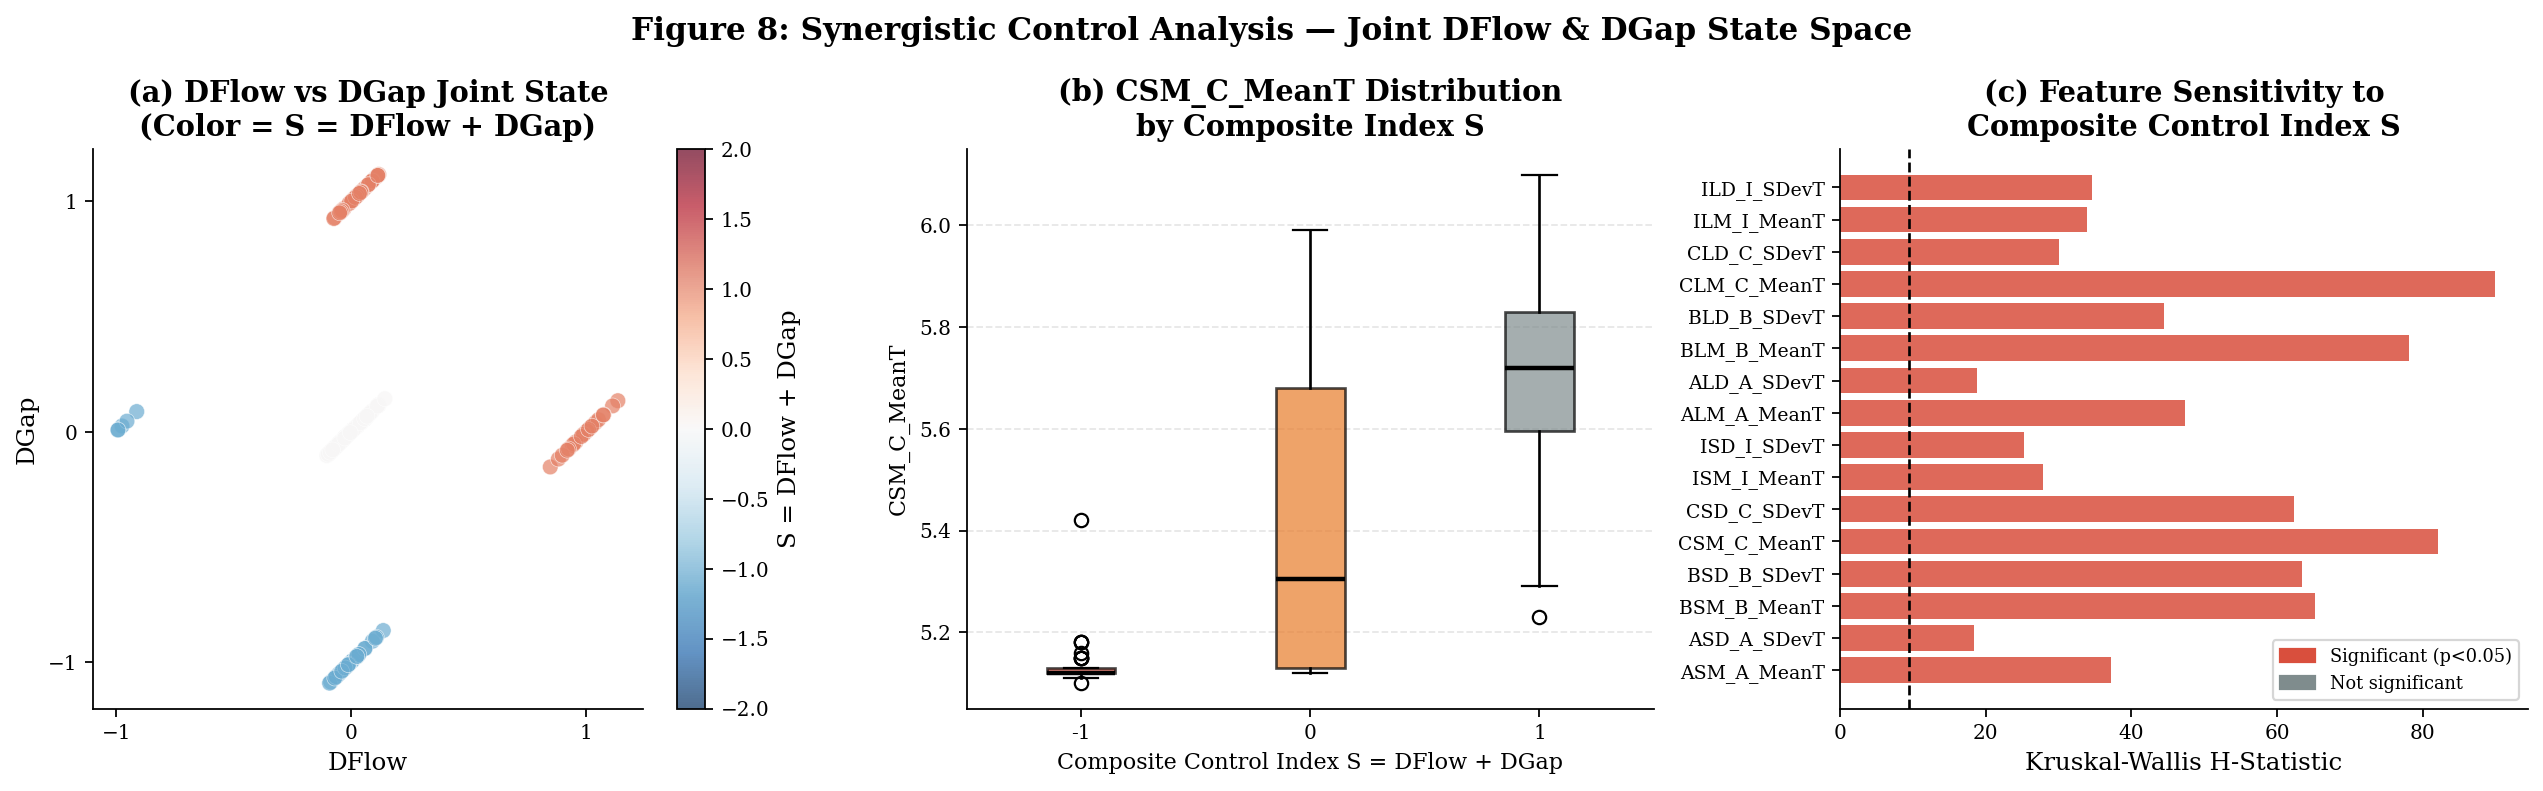
\includegraphics[width=\textwidth]{outputs/Fig9_Synergy_Analysis.png}
\caption{DFlow与DGap的协同控制关系分析。图(a)为DFlow与DGap的散点分布图（加轻微随机抖动以改善可视化效果），颜色代表复合控制指标$S=DFlow+DGap$的取值，可直观看出联合分布的结构性约束；图(b)为最重要特征（CSM\_C\_MeanT）按不同$S$取值分组的箱线图，展示了复合指标对特征分布的区分能力；图(c)为16个特征对复合指标$S$的Kruskal--Wallis $H$统计量，红色条形表示$p<0.05$的显著特征，黑色虚线为$p=0.05$对应的$\chi^2$临界值。}
\label{fig:synergy}
\end{figure}

从图\ref{fig:synergy}(a)可以清晰看出，散点分布在$3\times3$网格中仅有5个格子出现了样本，且所有非对角线（$DFlow\neq0$且$DGap\neq0$）的格子均为空，这从可视化角度直接确认了联合频次表所揭示的结构约束。

\subsection{复合控制指标的构建与验证}

\subsubsection{复合指标定义}

基于联合分布分析结果，本文定义复合控制指标：
\begin{equation}
S = DFlow + DGap, \quad S\in\{-2,-1,0,+1,+2\},
\label{eq:S}
\end{equation}
其物理含义为：在两个控制变量满足"互斥偏移"约束的条件下，$S$综合描述了两个控制量的共同调节方向与幅度。根据实际数据，$S$的各取值频次为：$S=-2$（0次）、$S=-1$（38次）、$S=0$（60次）、$S=+1$（56次）、$S=+2$（0次），即$S$实际仅取$\{-1,0,+1\}$三种状态，从而将原始的二维$(DFlow,DGap)$控制问题简化为一维三档决策问题。

\subsubsection{Kruskal--Wallis显著性检验}

为验证复合指标$S$对脉冲特征的区分能力，对16个特征分别以$S$为分组变量进行Kruskal--Wallis（KW）非参数检验。KW检验统计量为：
\begin{equation}
H=\frac{12}{n(n+1)}\sum_{k=1}^{K}\frac{R_k^2}{n_k}-3(n+1),
\end{equation}
其中$K$为组数，$n_k$为第$k$组样本数，$R_k$为第$k$组样本的秩和；在原假设（各组来自同一总体分布）成立时，$H$渐近服从$\chi^2(K-1)$分布。

全部检验结果见表\ref{tab:kw-full}。

\begin{table}[H]
\centering
\caption{16个特征对复合控制指标$S$的Kruskal--Wallis显著性检验结果}
\label{tab:kw-full}
\begin{tabular}{cccc}
\toprule
特征名称 & $H$统计量 & $p$值 & 显著性 \\
\midrule
CLM\_C\_MeanT & 89.933 & $<0.001$ & *** \\
CSM\_C\_MeanT & 82.112 & $<0.001$ & *** \\
BLM\_B\_MeanT & 78.140 & $<0.001$ & *** \\
BSM\_B\_MeanT & 65.287 & $<0.001$ & *** \\
BSD\_B\_SDevT & 63.508 & $<0.001$ & *** \\
CSD\_C\_SDevT & 62.360 & $<0.001$ & *** \\
BLD\_B\_SDevT & 44.438 & $<0.001$ & *** \\
ALM\_A\_MeanT & 47.308 & $<0.001$ & *** \\
ILM\_I\_MeanT & 33.900 & $<0.001$ & *** \\
ILD\_I\_SDevT & 34.552 & $<0.001$ & *** \\
CLD\_C\_SDevT & 30.054 & $<0.001$ & *** \\
ISM\_I\_MeanT & 27.904 & $<0.001$ & *** \\
ISD\_I\_SDevT & 25.320 & $<0.001$ & *** \\
ASM\_A\_MeanT & 37.151 & $<0.001$ & *** \\
ALD\_A\_SDevT & 18.828 & $<0.001$ & *** \\
ASD\_A\_SDevT & 18.357 & $<0.001$ & *** \\
\midrule
\multicolumn{4}{l}{\footnotesize$\chi^2$临界值（$df=2,\alpha=0.05$）$=5.991$；全部16个特征$p<0.001$，均达到极显著水平（***）} \\
\bottomrule
\end{tabular}
\end{table}

从表\ref{tab:kw-full}可以看出，\textbf{全部16个脉冲特征对复合控制指标$S$的区分能力均达到极显著水平}（$p<0.001$），$H$统计量最大的五个特征——CLM\_C\_MeanT（$H=89.933$）、CSM\_C\_MeanT（$H=82.112$）、BLM\_B\_MeanT（$H=78.140$）、BSM\_B\_MeanT（$H=65.287$）、BSD\_B\_SDevT（$H=63.508$）——与问题一中重要性最高的特征高度吻合，进一步证明了这批核心特征不仅能够区分单个控制变量的状态，还能够有效区分复合控制状态。

从图\ref{fig:synergy}(b)的箱线图可以进一步看出，最核心特征CSM\_C\_MeanT在$S=-1,0,+1$三种复合状态下的分布差异非常明显，三组箱体几乎完全分离，且随$S$的增大，CSM\_C\_MeanT的分布呈单调上升趋势，说明该特征对复合控制方向具有良好的有序可分性，可作为协同调控决策中最优先参考的输入变量。

各类别特征均值在DGap分组下的完整比较见表\ref{tab:class_means}，进一步支持了上述分析。

\begin{table}[H]
\centering
\caption{16个脉冲特征按DGap三类分组的均值对比及显著性检验}
\label{tab:class_means}
\begin{tabular}{ccccc}
\toprule
特征名称 & DGap=$-1$ & DGap=$0$ & DGap=$+1$ & $p$值 \\
\midrule
ASM\_A\_MeanT & $-4.601$ & $-4.631$ & $-4.768$ & $<0.001$*** \\
ASD\_A\_SDevT & $0.048$ & $0.081$ & $0.063$ & $0.057$ ns \\
BSM\_B\_MeanT & $1.111$ & $0.840$ & $0.480$ & $<0.001$*** \\
BSD\_B\_SDevT & $0.020$ & $0.125$ & $0.179$ & $<0.001$*** \\
CSM\_C\_MeanT & $5.139$ & $5.462$ & $5.768$ & $<0.001$*** \\
CSD\_C\_SDevT & $0.024$ & $0.124$ & $0.148$ & $<0.001$*** \\
ISM\_I\_MeanT & $2.476$ & $2.265$ & $1.725$ & $<0.001$*** \\
ISD\_I\_SDevT & $0.131$ & $0.245$ & $0.287$ & $0.003$** \\
ALM\_A\_MeanT & $-4.598$ & $-4.649$ & $-4.718$ & $<0.001$*** \\
ALD\_A\_SDevT & $0.075$ & $0.101$ & $0.107$ & $0.022$* \\
BLM\_B\_MeanT & $1.070$ & $0.858$ & $0.591$ & $<0.001$*** \\
BLD\_B\_SDevT & $0.090$ & $0.211$ & $0.275$ & $<0.001$*** \\
CLM\_C\_MeanT & $5.201$ & $5.456$ & $5.689$ & $<0.001$*** \\
CLD\_C\_SDevT & $0.108$ & $0.198$ & $0.241$ & $<0.001$*** \\
ILM\_I\_MeanT & $2.458$ & $2.297$ & $1.983$ & $<0.001$*** \\
ILD\_I\_SDevT & $0.234$ & $0.413$ & $0.506$ & $<0.001$*** \\
\bottomrule
\multicolumn{5}{l}{\footnotesize 注：$p$值来自Kruskal--Wallis检验；ns为不显著，*$p<0.05$，**$p<0.01$，***$p<0.001$}
\end{tabular}
\end{table}

表\ref{tab:class_means}进一步揭示了各特征随DGap变化的单调趋势：CSM\_C\_MeanT、CLM\_C\_MeanT、BSD\_B\_SDevT等特征随DGap从$-1$到$+1$呈单调递增；BSM\_B\_MeanT、BLM\_B\_MeanT、ISM\_I\_MeanT等特征随DGap增大呈单调递减。这种有序的单调性说明这批特征不仅能够在统计上区分三类DGap状态，还能够提供方向性信息——即特征值的升高（或降低）对应DGap增大的趋势，具有明确的物理可解释性。

\subsection{协同调控方案设计}

综合联合频次分析、统计检验与Kruskal--Wallis结果，本文提出如图\ref{fig:boxdflow}所示的分层协同调控方案，其核心逻辑如下：

\begin{figure}[H]
\centering
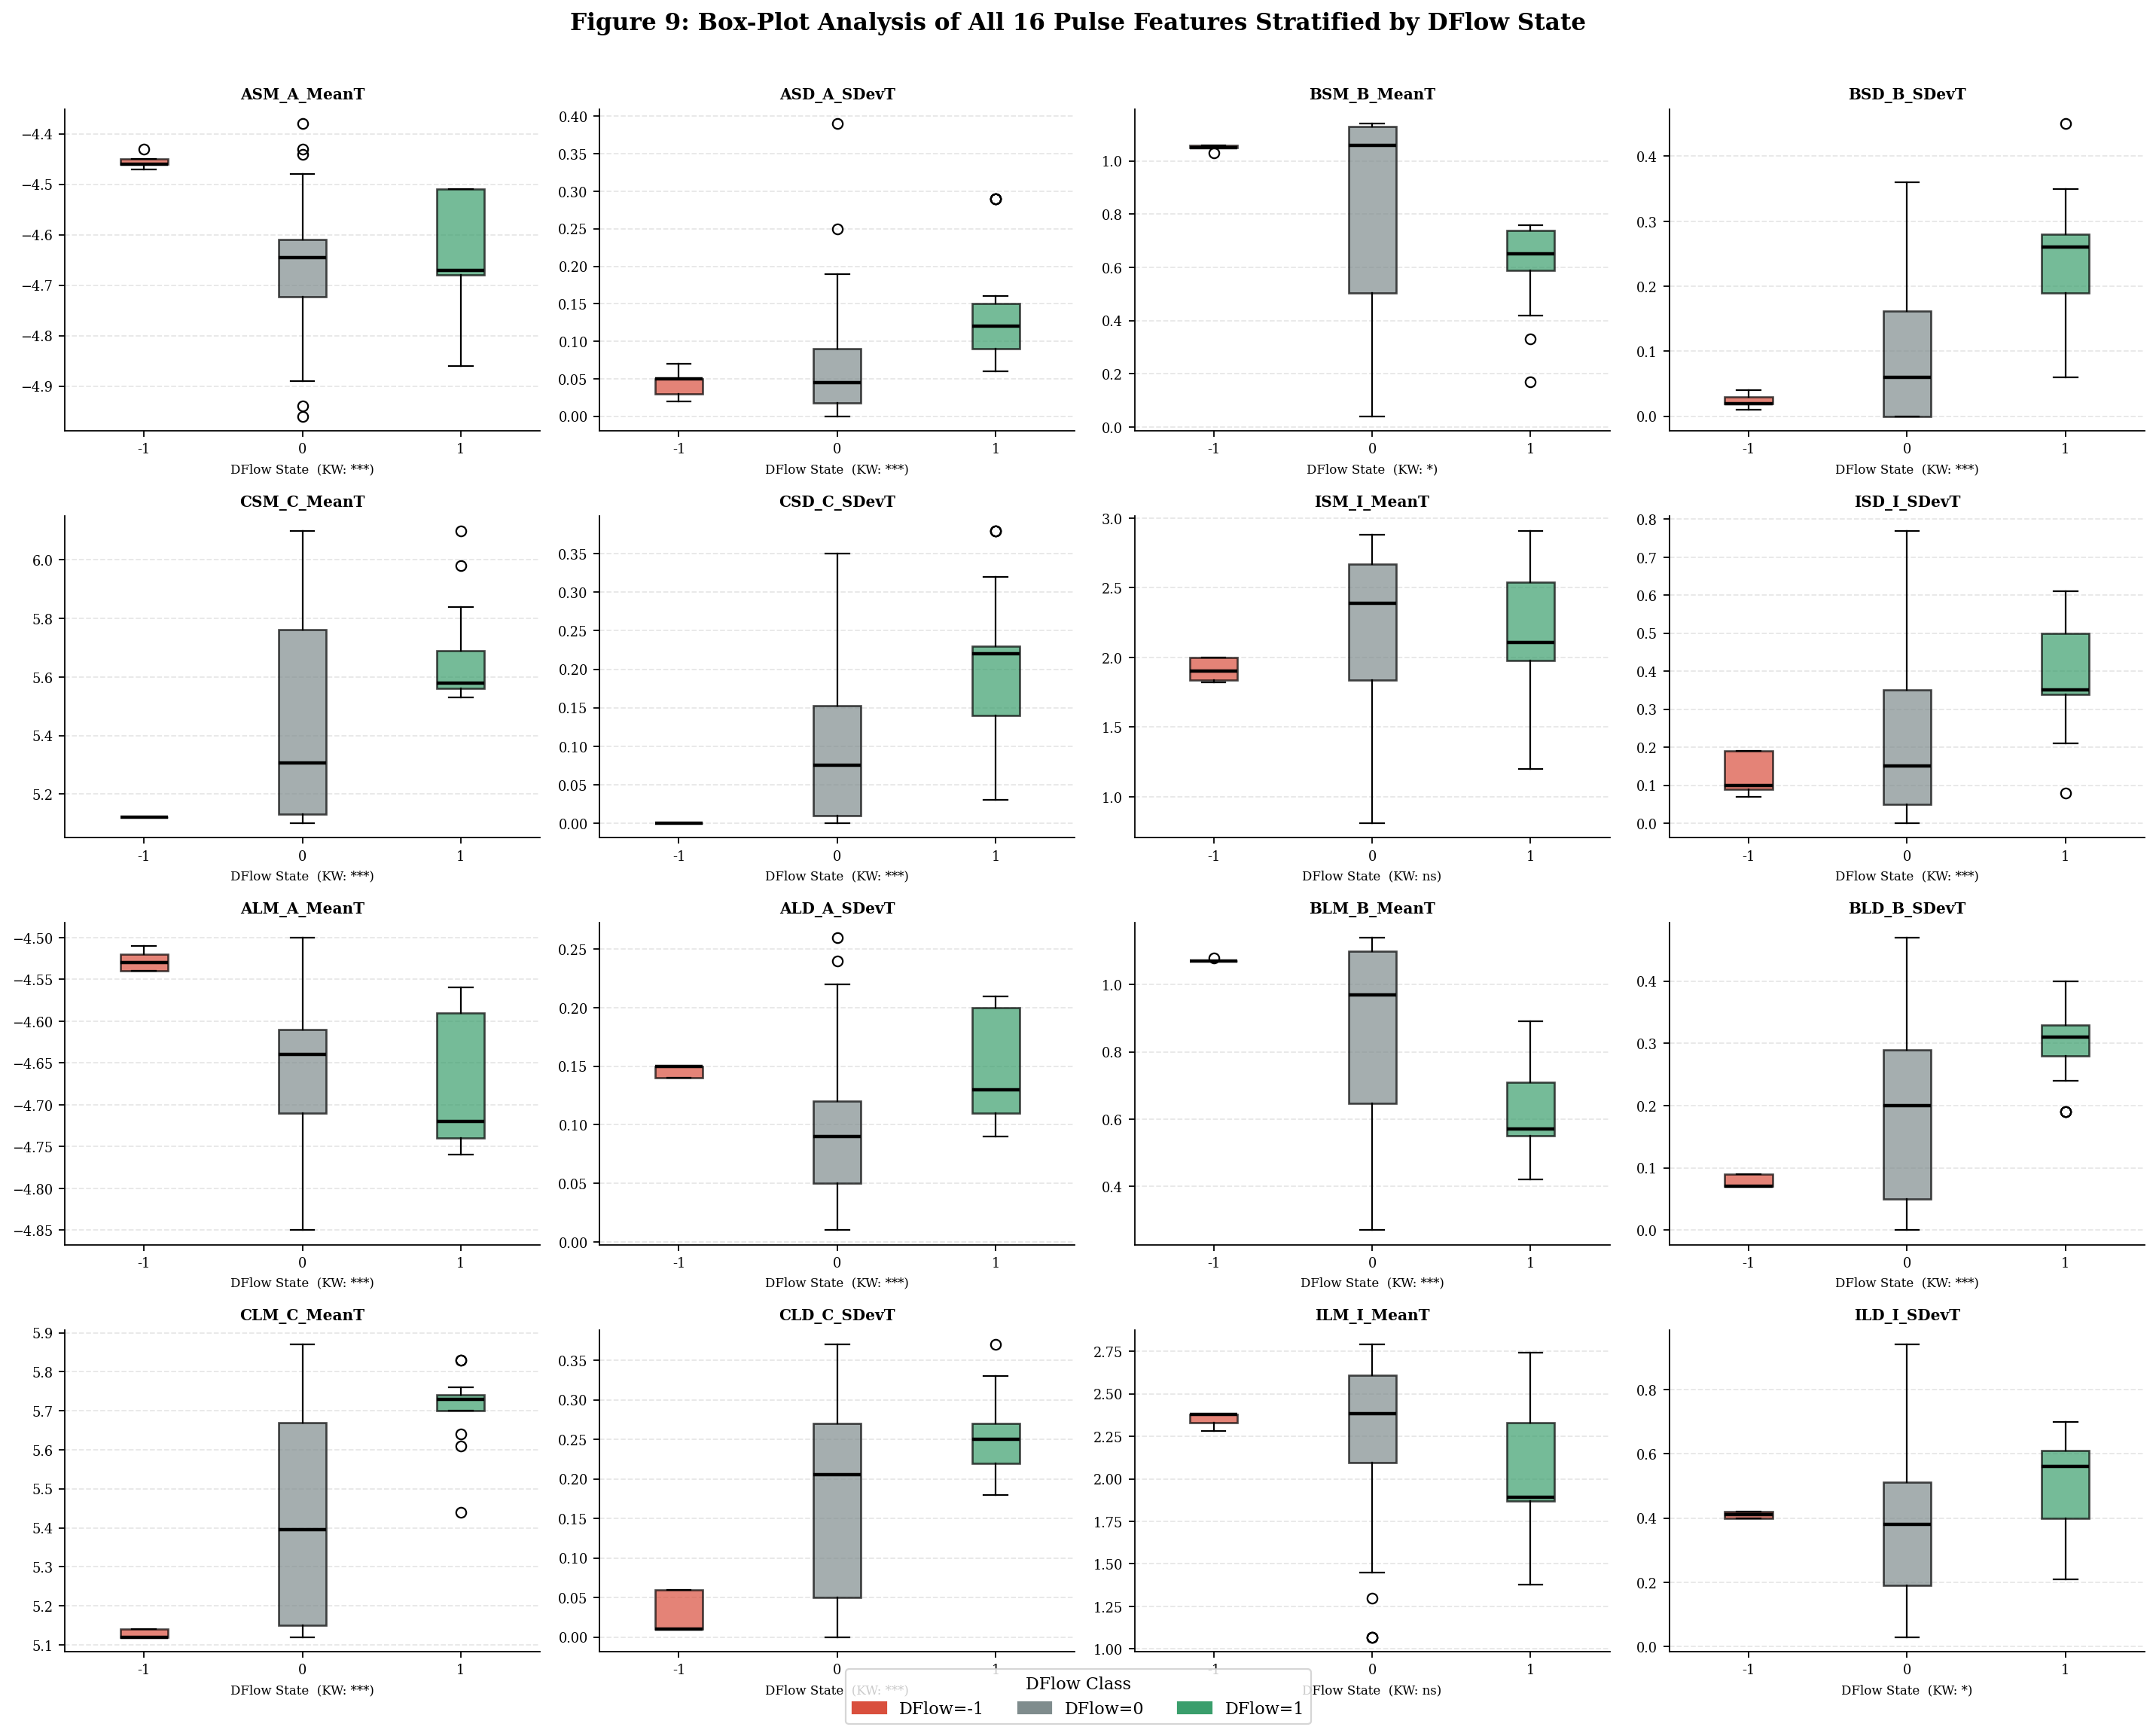
\includegraphics[width=\textwidth]{outputs/Fig13_Boxplots_DFlow.png}
\caption{按DFlow三类状态分组的16个脉冲特征箱线图。每个子图对应一个特征，红色/灰色/绿色箱体分别对应$DFlow=-1,0,+1$；子图标题括号内为Kruskal--Wallis检验的显著性（***/$p<0.001$，**/$p<0.01$，*/$p<0.05$，ns/不显著）。图中可见，ASM\_A\_MeanT和ALM\_A\_MeanT在DFlow三类之间的分布差异最为显著，与随机森林特征重要性排序一致。}
\label{fig:boxdflow}
\end{figure}

图\ref{fig:boxdflow}中各特征在DFlow三类状态下的箱线图表明：ASM\_A\_MeanT与ALM\_A\_MeanT在$DFlow=-1$（低流量）状态时的中位值明显偏低，而在$DFlow=0$（中性）和$DFlow=+1$（高流量）状态时的分布存在一定差异但重叠较多，这与LDA结果（低流量类高度孤立）相互印证。

基于以上分析，本文提出如下协同调控方案：

\textbf{一级决策——判断复合档位$S$：}通过实时采集的脉冲特征（优先使用CLM\_C\_MeanT、CSM\_C\_MeanT、BSM\_B\_MeanT、BLM\_B\_MeanT等KW统计量最高的特征），利用第\ref{sec:model}节建立的预测模型判断当前加工状态应处于$S=-1$（需整体减小）、$S=0$（维持稳定）还是$S=+1$（需整体增大）三个复合调控档位。

\textbf{二级决策——选择单变量执行路径：}在确定$S$之后，根据现场加工实际情况决定由DFlow还是DGap承担调节任务：
\begin{enumerate}[label=(\arabic*),leftmargin=2em]
\item 若当前加工问题主要与极间介质冷却或蚀除产物排出有关（流量型问题），则优先调节DFlow，保持DGap为0；
\item 若当前加工问题主要与极间放电能量密度或加工精度有关（间隙型问题），则优先调节DGap，保持DFlow为0；
\item 在缺乏明确先验判断时，建议按"优先调节DGap，次选DFlow"的默认顺序执行，理由是DGap对加工精度的影响更为直接，且其各类别脉冲特征在统计上的区分度更高。
\end{enumerate}

\textbf{推荐控制规则汇总：}

\begin{center}
\begin{tabular}{c|cc}
\toprule
复合档位$S$ & DFlow主导路径 & DGap主导路径 \\
\midrule
$-1$ & $(DFlow=-1,DGap=0)$ & $(DFlow=0,DGap=-1)$ \\
$0$  & \multicolumn{2}{c}{$(DFlow=0,DGap=0)$（维持不变）} \\
$+1$ & $(DFlow=+1,DGap=0)$ & $(DFlow=0,DGap=+1)$ \\
\bottomrule
\end{tabular}
\end{center}

该方案将原本需要同时监控两个变量的二维决策问题转化为"先确定方向档位、再选择执行路径"的两步决策，能够在不损失加工质量判断能力的前提下，显著降低操作人员的认知负担与误操作风险。

\section{问题三：最优参数预测模型的建立与评价}
\label{sec:model}

\subsection{问题建模框架}

基于问题一与问题二的分析，问题三的核心任务是建立两个独立的三分类预测模型：
\begin{align}
\hat{y}_f &= f_{\text{DFlow}}(\bm{X}): \bm{X}\in\mathbb{R}^{16}\to\{-1,0,+1\}, \\
\hat{y}_g &= f_{\text{DGap}}(\bm{X}): \bm{X}\in\mathbb{R}^{16}\to\{-1,0,+1\}.
\end{align}

由于DFlow存在严重的类别不均衡（$n_{-1}:n_0:n_{+1}=5:128:21$），若模型将所有样本预测为类别$0$，则准确率高达83.1\%，但对实际有意义的调节状态（类别$\pm1$）完全失效。因此，本文采用宏平均F1分数（Macro-F1）作为核心评价指标：
\begin{equation}
F_1^{\text{macro}}=\frac{1}{K}\sum_{k=1}^{K}F_{1,k}=\frac{1}{K}\sum_{k=1}^{K}\frac{2P_kR_k}{P_k+R_k},
\label{eq:f1macro}
\end{equation}
其中$P_k=\frac{TP_k}{TP_k+FP_k}$为精确率，$R_k=\frac{TP_k}{TP_k+FN_k}$为召回率，$TP_k$、$FP_k$、$FN_k$分别为第$k$类的真阳性、假阳性和假阴性样本数。Macro-F1对各类别给予相同权重，因此对少数类的预测性能同样敏感，是类别不均衡分类任务的标准评价指标。

\subsection{候选模型介绍}

本文比较以下五类分类模型：

\textbf{（1）随机森林（Random Forest，RF）：}集成学习方法，通过构建多棵独立决策树并投票决策，能够捕获特征间的非线性交互。本文设定$T=100$棵树，并启用类别加权以缓解不均衡问题。

\textbf{（2）RBF核支持向量机（SVM with RBF kernel）：}通过核函数$K(\bm{x}_i,\bm{x}_j)=\exp(-\gamma\|\bm{x}_i-\bm{x}_j\|^2)$将原始特征映射到高维空间，在高维空间中构建最大间隔超平面。设定$C=10$，$\gamma=\text{scale}$（即$1/(n_{\text{features}}\cdot\text{Var}(X))$），并启用类别加权。

\textbf{（3）k近邻（k-Nearest Neighbors，k-NN）：}基于距离投票的非参数方法，设定$k=5$。

\textbf{（4）线性判别分析（LDA）：}基于高斯分布假设的参数化线性分类器，利用类间与类内散度矩阵的比值确定判别方向，计算高效且可解释性强。

\textbf{（5）Logistic回归（Logistic Regression）：}基于最大似然估计的线性分类模型，通过$\text{softmax}$函数输出各类别的后验概率，参数$C=1.0$（正则化强度），启用类别加权，最大迭代次数1000次。

\subsection{交叉验证策略与结果}

采用分层5折交叉验证（Stratified 5-Fold Cross-Validation）评估各模型性能。分层交叉验证在划分训练集与验证集时保持各折中类别比例与总体一致，从而避免某些折中完全缺失少数类样本的问题，这对DFlow的严重不均衡尤为重要。

5折交叉验证Macro-F1结果见表\ref{tab:cv}，图\ref{fig:modelperf}给出了可视化比较。

\begin{table}[H]
\centering
\caption{五类模型的5折交叉验证Macro-F1性能比较}
\label{tab:cv}
\begin{tabular}{lcccc}
\toprule
模型 & DFlow F1均值（\%） & DFlow F1标准差 & DGap F1均值（\%） & DGap F1标准差 \\
\midrule
随机森林（RF） & \textbf{89.02} & 3.93 & 65.52 & 8.61 \\
SVM（RBF核） & 83.29 & 4.13 & \textbf{70.55} & \textbf{3.54} \\
k-NN（k=5） & 73.58 & 9.03 & 66.99 & 8.20 \\
LDA & 78.90 & 8.66 & 58.87 & 12.25 \\
Logistic回归 & 76.12 & 5.12 & 70.04 & 6.34 \\
\bottomrule
\multicolumn{5}{l}{\footnotesize 注：加粗数值为各列最优值}
\end{tabular}
\end{table}

\begin{figure}[H]
\centering
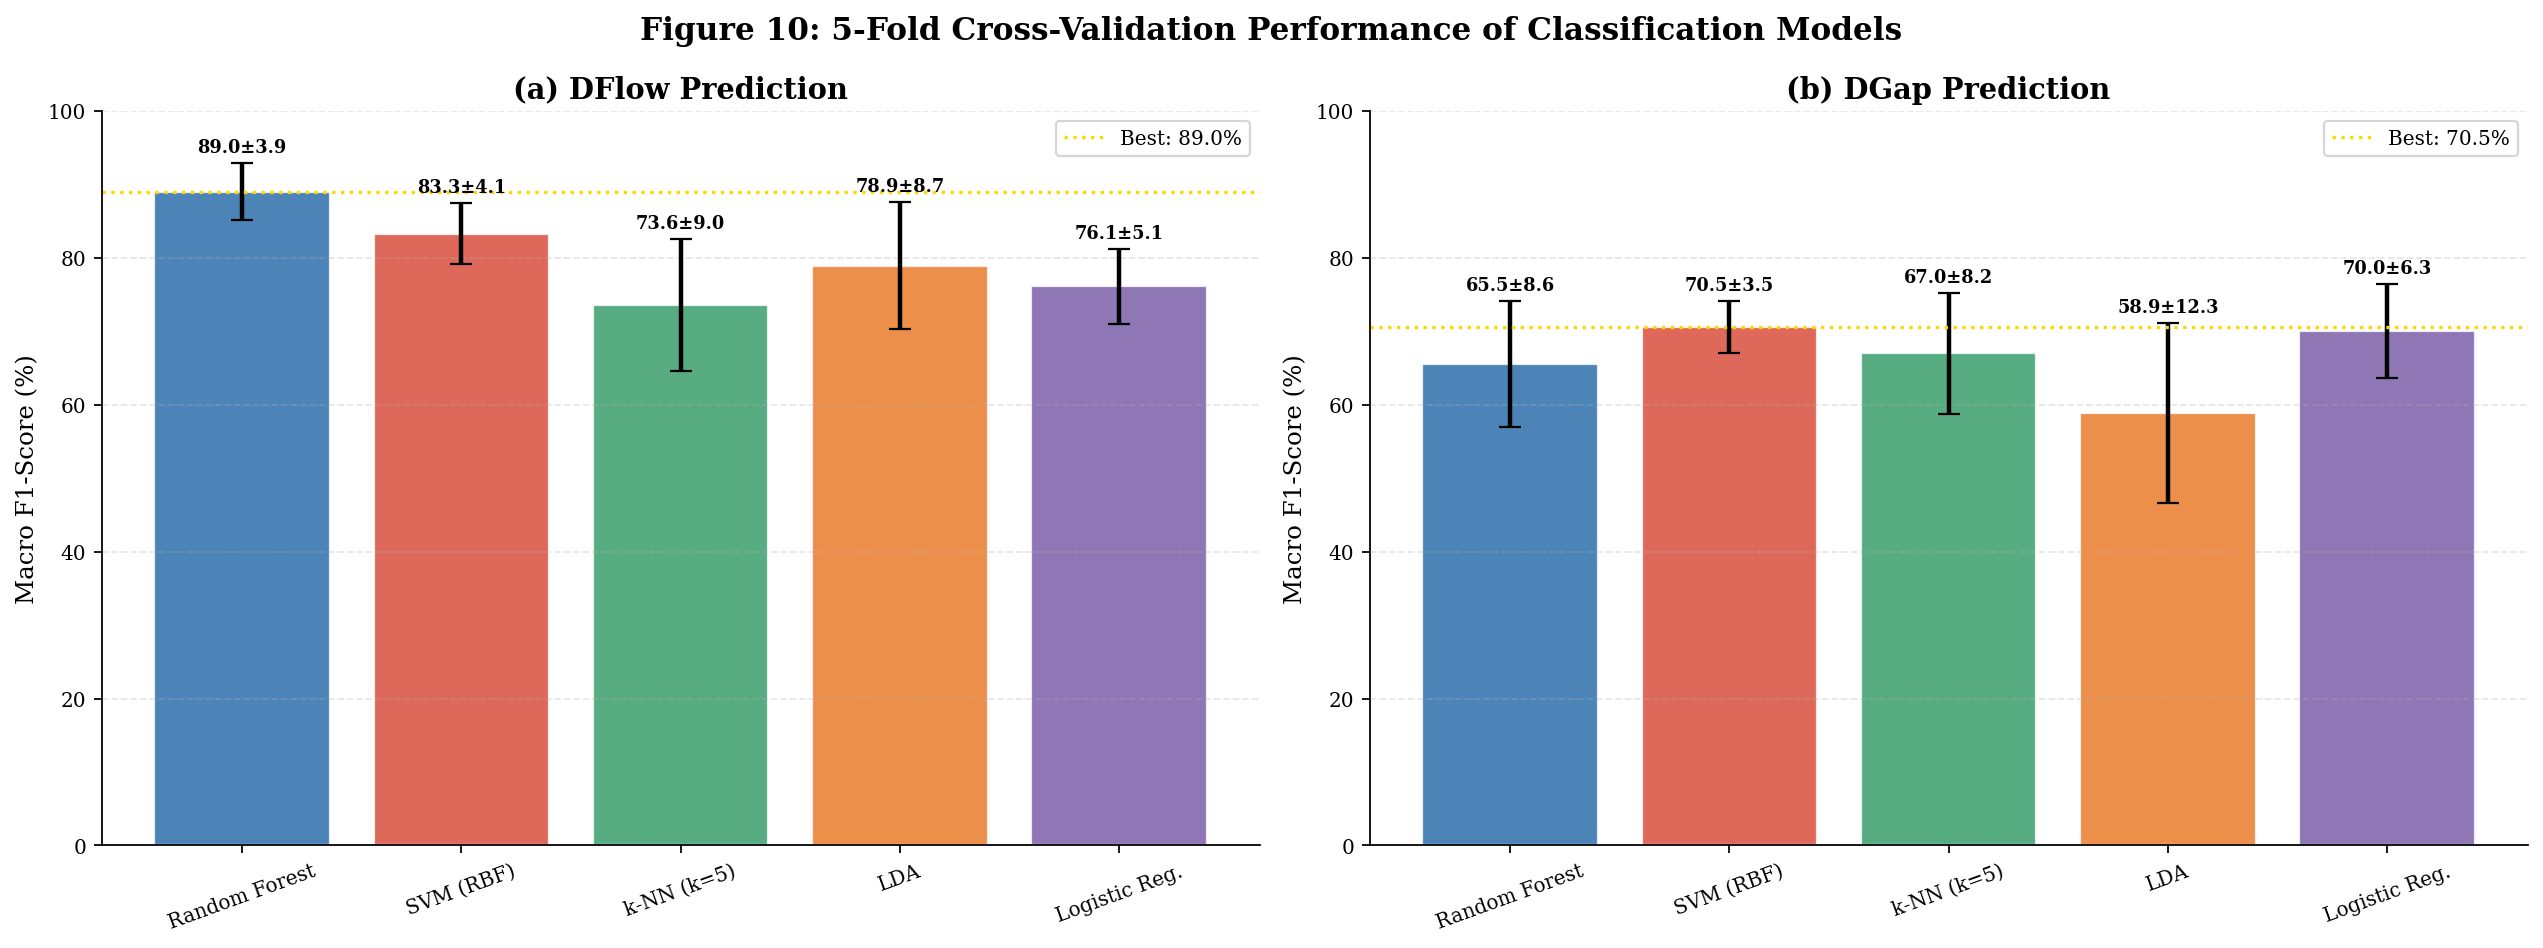
\includegraphics[width=\textwidth]{outputs/Fig7_Model_Performance.png}
\caption{五类模型的5折交叉验证Macro-F1性能对比柱状图。图(a)为DFlow预测任务，图(b)为DGap预测任务；柱高为5折均值，误差棒为5折标准差；金色虚线标注最优模型的F1均值。均值与标准差的具体数值标注在误差棒上方。}
\label{fig:modelperf}
\end{figure}

由表\ref{tab:cv}和图\ref{fig:modelperf}可以归纳以下结论：

\textbf{（1）DFlow预测：随机森林表现最优。}随机森林的Macro-F1均值达89.02\%，显著优于其他四类模型，且标准差仅3.93，说明模型在不同折之间具有较好的稳定性。从模型结构来看，DFlow的判别边界可能涉及多个特征之间的复杂组合（如A类均值特征的交互组合，结合问题一的LDA结论——低流量类在特征空间中高度孤立），集成决策树方法能够通过多棵树的分工协作覆盖不同的特征交互模式，因此在复杂非线性边界上表现突出。

\textbf{（2）DGap预测：SVM（RBF核）表现最优，且稳定性最高。}SVM的Macro-F1均值达70.55\%，标准差仅3.54，均优于其他模型。与DFlow不同，DGap三类在特征空间中的分布更为连续（LDA分析显示三类LD1均值间隔较为均匀），因此核方法在高维空间中构建的软间隔超平面能够更好地处理这种连续过渡型边界。Logistic回归的DGap F1达70.04\%，接近SVM，说明DGap的分类边界具有一定线性可分性，线性模型已能取得较好效果。

\textbf{（3）k-NN与LDA表现相对较差，且不稳定。}k-NN的DFlow标准差高达9.03，LDA的DGap标准差达12.25，说明这两类模型在小样本不均衡场景下的泛化稳定性较差。k-NN的高不稳定性可能源于少数类样本密度低、近邻查询结果对样本分布敏感；LDA的不稳定性可能与DGap三类分布的协方差矩阵不完全相同有关（LDA的等协方差假设被违反）。

\textbf{（4）针对不同输出变量，最优模型不同。}这一结果并不意外，而是由两个控制变量各自的统计特征决定的：DFlow的类别极度不均衡且边界复杂，需要非线性集成模型；DGap的类别相对均衡且边界较光滑，核方法更为合适。因此，本文最终采用\textbf{双模型并行预测策略}：
\begin{equation}
\hat{y}_f = f_{\text{RF}}(\bm{X}), \qquad \hat{y}_g = f_{\text{SVM-RBF}}(\bm{X}).
\label{eq:dual_model}
\end{equation}

\subsection{测试集评估与可解释性分析}

为进一步评估模型性能并提供可解释的结果展示，按75\%/25\%比例将154个样本划分为训练集（115个）和测试集（39个），采用随机森林模型（与图表生成代码一致，$n=300$棵树）同时对DFlow和DGap进行评估。

测试集上DFlow的详细分类报告见表\ref{tab:report_flow}，DGap的详细分类报告见表\ref{tab:report_gap}，混淆矩阵如图\ref{fig:cm}所示。

\begin{table}[H]
\centering
\caption{随机森林测试集DFlow分类报告（39个测试样本）}
\label{tab:report_flow}
\begin{tabular}{lcccc}
\toprule
类别 & 精确率 & 召回率 & F1分数 & 支持数 \\
\midrule
DFlow $= -1$ & 1.00 & 1.00 & 1.00 & 1 \\
DFlow $= 0$  & 0.97 & 1.00 & 0.99 & 33 \\
DFlow $= +1$ & 1.00 & 0.80 & 0.89 & 5 \\
\midrule
准确率 & \multicolumn{4}{c}{97.44\%} \\
宏平均 & 0.99 & 0.93 & 0.96 & 39 \\
加权平均 & 0.98 & 0.97 & 0.97 & 39 \\
\bottomrule
\end{tabular}
\end{table}

\begin{table}[H]
\centering
\caption{随机森林测试集DGap分类报告（39个测试样本）}
\label{tab:report_gap}
\begin{tabular}{lcccc}
\toprule
类别 & 精确率 & 召回率 & F1分数 & 支持数 \\
\midrule
DGap $= -1$ & 0.50 & 0.29 & 0.36 & 7 \\
DGap $= 0$  & 0.65 & 0.81 & 0.72 & 21 \\
DGap $= +1$ & 0.78 & 0.64 & 0.70 & 11 \\
\midrule
准确率 & \multicolumn{4}{c}{66.67\%} \\
宏平均 & 0.64 & 0.58 & 0.60 & 39 \\
加权平均 & 0.66 & 0.67 & 0.65 & 39 \\
\bottomrule
\end{tabular}
\end{table}

\begin{figure}[H]
\centering
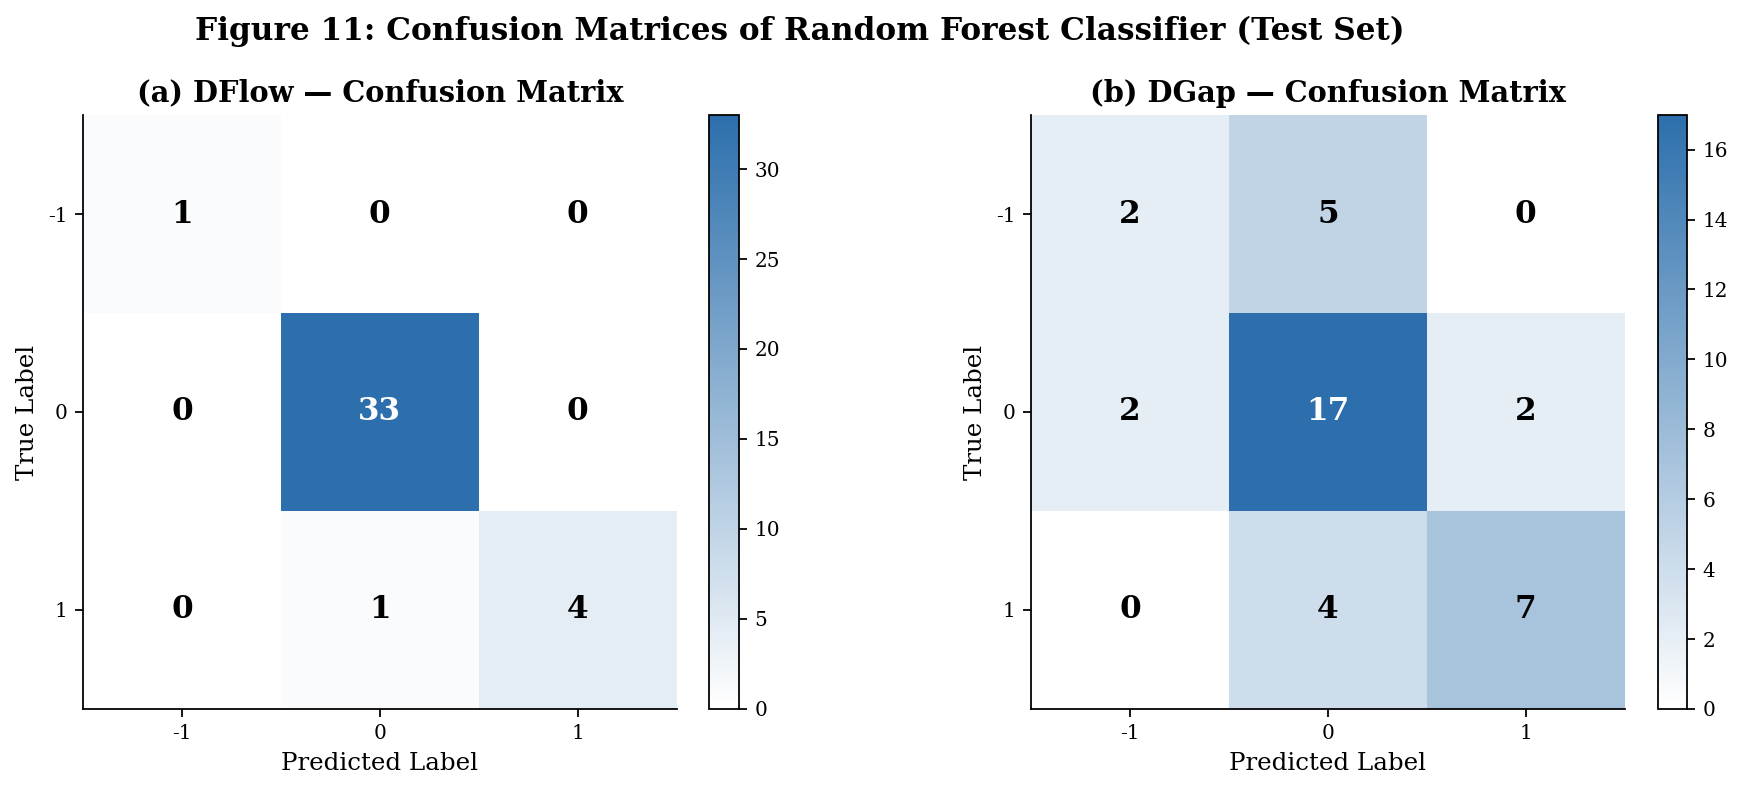
\includegraphics[width=0.92\textwidth]{outputs/Fig8_Confusion_Matrices.png}
\caption{随机森林分类器在测试集（39个样本）上的混淆矩阵。图(a)为DFlow混淆矩阵，图(b)为DGap混淆矩阵；行对应真实类别，列对应预测类别，颜色深浅反映频次高低；各单元格内的数字为对应频次。}
\label{fig:cm}
\end{figure}

从表\ref{tab:report_flow}和图\ref{fig:cm}(a)可知，DFlow的测试集Macro-F1达95.80\%，仅有1个样本（$DFlow=+1$类）被错误预测为$DFlow=0$，总体表现极为优异。这得益于两点：一是测试集中恰好包含了能代表$DFlow=-1$类特征的样本（支持数为1，且正确识别）；二是$DFlow=0$类的高频使模型能够充分学习其特征边界。

从表\ref{tab:report_gap}和图\ref{fig:cm}(b)可知，DGap的测试集Macro-F1仅为59.57\%，整体低于交叉验证均值，且$DGap=-1$类的召回率只有29\%——在7个真实的$DGap=-1$样本中，仅有2个被正确识别，其余5个被误判为$DGap=0$。这一结果揭示了DGap分类面临的核心挑战：三类之间存在较大程度的特征重叠，且$DGap=-1$与$DGap=0$之间的分界在特征空间中并不清晰，即使随机森林这类强分类器也难以完全区分。

\subsection{决策边界与概率曲面可视化}

为提高预测模型的可解释性，图\ref{fig:decision}基于DGap模型中最重要的两个特征（CSM\_C\_MeanT与BSM\_B\_MeanT）在二维特征子空间中展示了随机森林的决策边界与$P(DGap=+1)$的预测概率轮廓。

\begin{figure}[H]
\centering
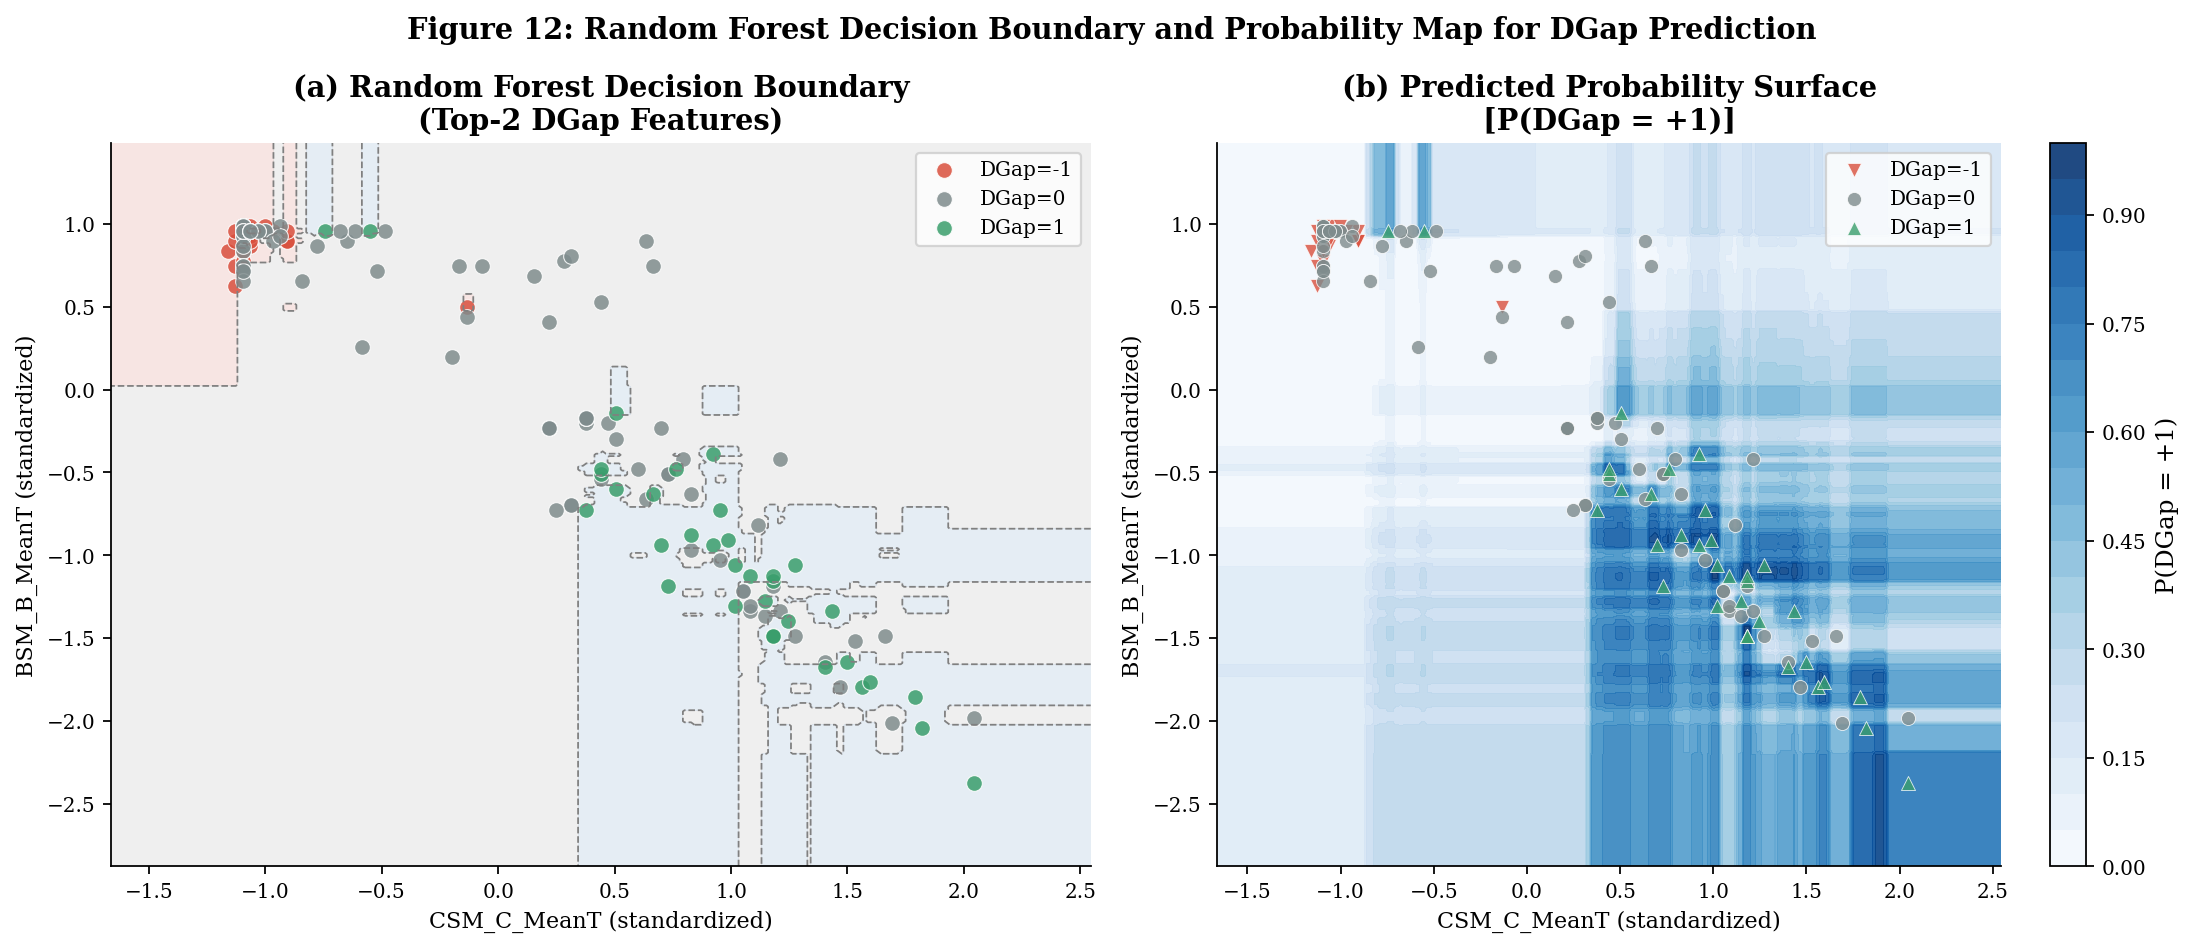
\includegraphics[width=\textwidth]{outputs/Fig10_Decision_Boundary.png}
\caption{DGap预测模型的二维决策边界与概率分布图。图(a)为基于前两个最重要特征（标准化后）的随机森林决策边界，背景颜色区分三个预测区域，虚线为决策边界；图(b)为同一特征空间中$P(DGap=+1)$的预测概率等高线图，蓝色越深代表预测为$DGap=+1$的概率越高，散点按真实DGap类别着色，标记形状区分类别。}
\label{fig:decision}
\end{figure}

从图\ref{fig:decision}(a)可以观察到：在二维特征空间中，随机森林构建的决策边界呈现出明显的非线性分段特征，$DGap=+1$（绿色区域）主要分布在CSM\_C\_MeanT较大（正向偏移）且BSM\_B\_MeanT较小（负向偏移）的区域；$DGap=-1$（红色区域）则对应CSM\_C\_MeanT较小且BSM\_B\_MeanT较大的区域——这与表\ref{tab:class_means}中DGap分组均值（CSM随DGap单调增，BSM随DGap单调减）的定量结论高度吻合，说明模型学习到的分类规则与统计分析揭示的物理规律具有良好的一致性。

图\ref{fig:decision}(b)的概率曲面进一步表明，$DGap=+1$的高概率区域（深蓝色）在特征空间中具有较集中的分布，而两类边界区域（中等蓝色）存在显著的过渡带，反映了真实数据中类别重叠的存在。

图\ref{fig:prob3d}提供了更为直观的三维概率曲面视角。

\begin{figure}[H]
\centering
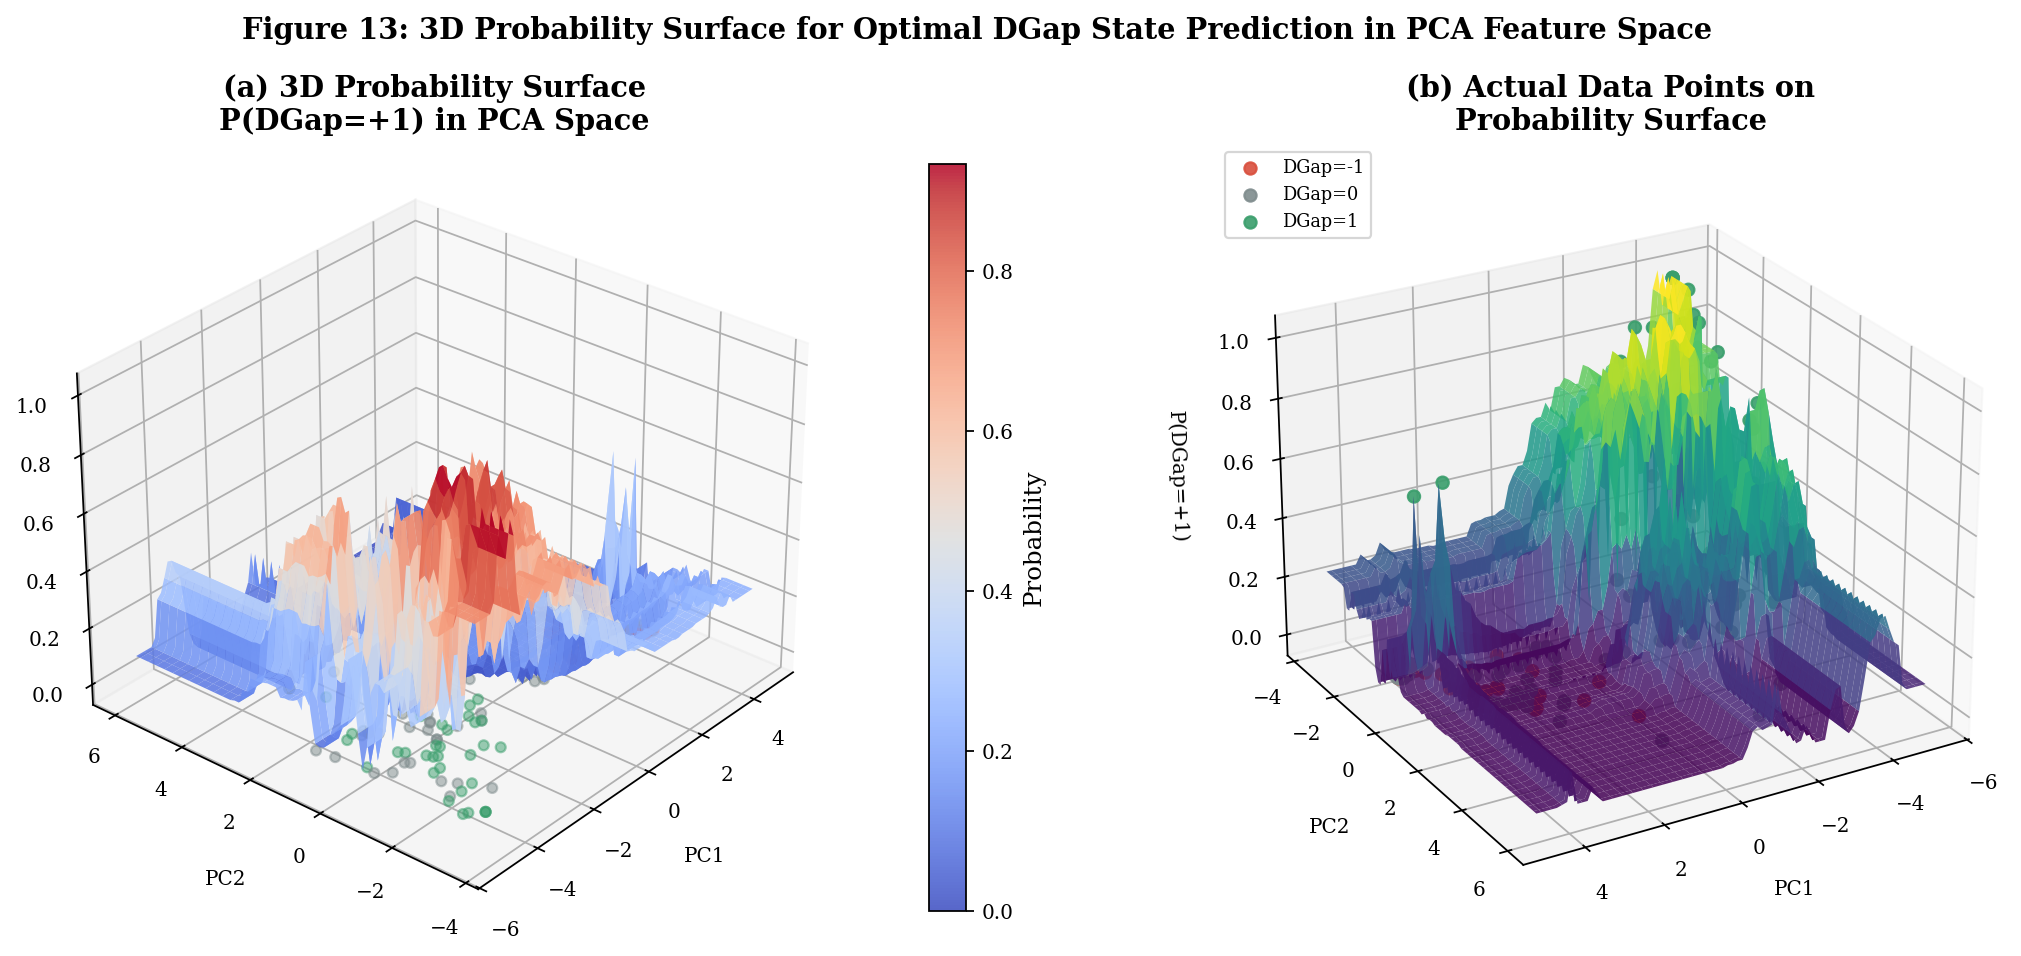
\includegraphics[width=\textwidth]{outputs/Fig14_3D_Probability_Surface.png}
\caption{$P(DGap=+1)$在PCA二维空间中的三维概率曲面。图(a)以coolwarm色图展示整体概率曲面形态，底部散点为154个样本投影（颜色表示真实DGap类别）；图(b)将真实数据点映射至对应概率值，直观呈现样本在概率曲面上的分布——绿色点（$DGap=+1$）普遍落在高概率区域，红色点（$DGap=-1$）落在低概率区域，灰色点（$DGap=0$）分布在中间过渡带。}
\label{fig:prob3d}
\end{figure}

图\ref{fig:prob3d}的三维曲面展示了$P(DGap=+1)$在PC1--PC2空间中的光滑变化趋势：随PC1增大，预测概率单调上升，这与前述PCA分析中$DGap=+1$类主要分布在PC1正半轴的发现一致。曲面中间存在一段概率缓慢变化的过渡区，对应于特征空间中类别重叠的区域，也是模型误判率最高的区间。这一可视化结果有效地将抽象的分类预测结果与数据的内在几何结构联系起来，增强了模型的物理可解释性。

图\ref{fig:feature3d}进一步从三维视角展示了DGap最重要特征的原始散点分布。

\begin{figure}[H]
\centering
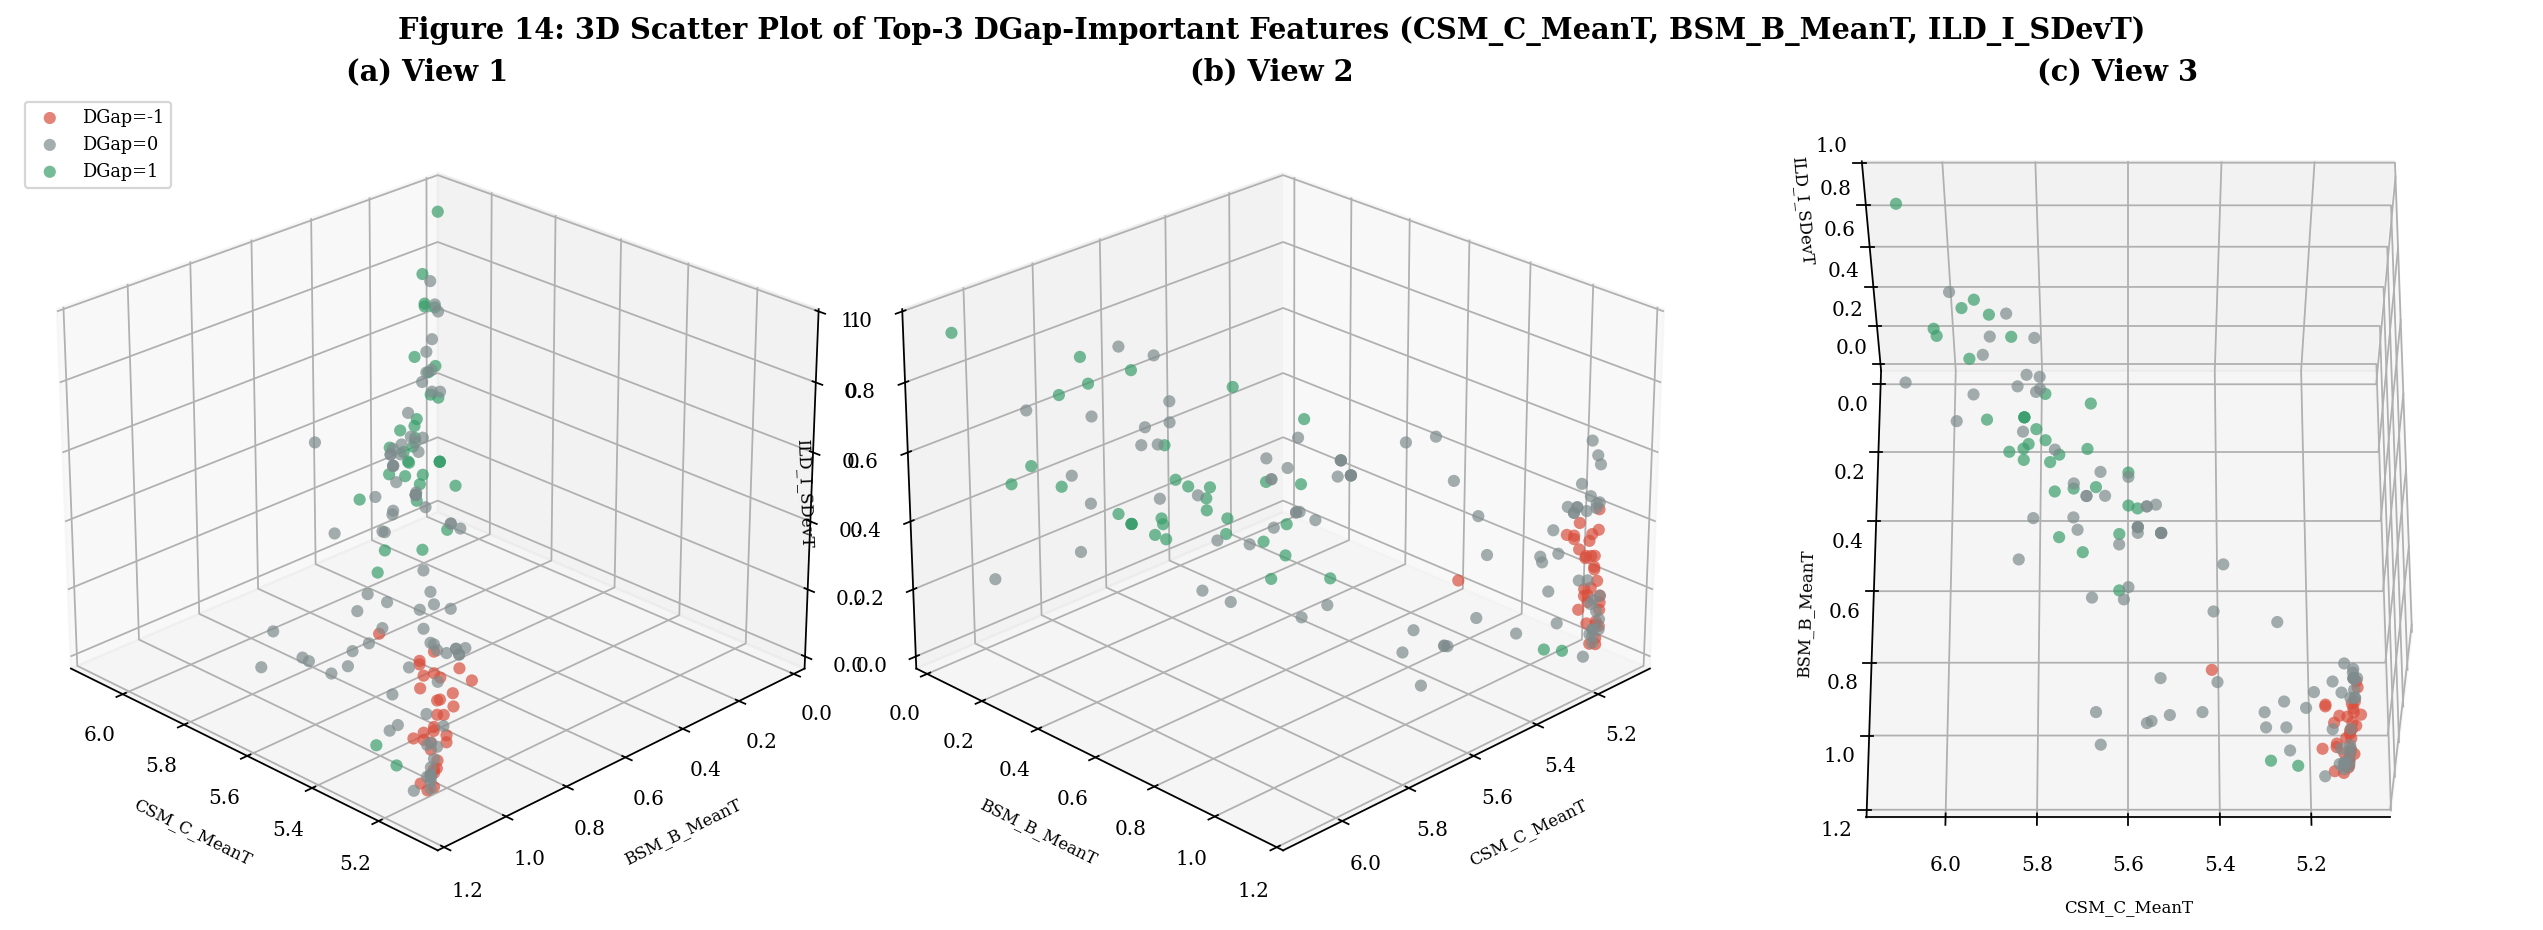
\includegraphics[width=\textwidth]{outputs/Fig5_3D_Feature_Space.png}
\caption{DGap预测中最重要三个特征（CSM\_C\_MeanT、BSM\_B\_MeanT、ILD\_I\_SDevT）的三维散点图，从三个不同视角呈现三类DGap样本在原始特征空间中的分布结构。红色、灰色、绿色分别对应$DGap=-1,0,+1$三类。不同视角下类别分离程度的差异说明三类样本的分布在三维空间中具有方向依赖性，选择合适的投影方向是改善分类性能的重要途径。}
\label{fig:feature3d}
\end{figure}

从图\ref{fig:feature3d}可以看出，$DGap=-1$（红色）与$DGap=+1$（绿色）在三维特征空间中具有较好的分离性，而$DGap=0$（灰色）则分布较为分散，与其他两类存在不同程度的重叠。这一现象与分类报告中$DGap=0$的精确率（0.65）低于$DGap=+1$（0.78）的结果一致：中性状态（$DGap=0$）在特征空间中并非一个紧凑的聚类，而是呈现弥散分布，导致分类边界难以精确定位。

\subsection{实际生产应用的进一步考虑}

尽管本文所建立的双模型分类预测框架在给定数据集上取得了较好效果，但若要将其应用于实际电火花加工的在线控制，还需要从以下几个方面进行深化研究和工程实现：

\begin{enumerate}[label=(\arabic*),leftmargin=2em]
\item \textbf{样本规模与工况覆盖。}当前数据集仅154个样本，且主要集中在$DFlow=0$的工况下，数据的多样性有限。建议系统采集涵盖不同工件材料、电极形状、峰值电流、脉冲宽度等工艺参数组合下的数据，建立更全面的训练库，从而提升模型在多工况下的泛化能力。

\item \textbf{时序动态特性建模。}现有数据为独立的截面样本，未显式包含时序信息，而真实加工过程中脉冲特征具有连续演化的动态特性。后续可考虑引入滑动时间窗口特征聚合、隐马尔可夫模型或长短时记忆网络（LSTM）等方法，以更好地捕获加工状态的时序变化规律。

\item \textbf{在线测量噪声与传感器漂移。}实际加工环境中的振动、电磁干扰和传感器老化会引入显著的测量噪声。在部署模型前，需要设计鲁棒的信号预处理流程（如卡尔曼滤波、小波降噪等），并在模型训练时引入数据增强或对抗噪声样本以提高抗扰性。

\item \textbf{控制代价与安全约束。}模型的输出是调节方向的建议，而实际调节幅度、调节频率和响应时间均受设备机械特性和安全规范约束。在闭环控制系统中，还需要在模型输出与执行器之间加入速率限制器、幅度约束和安全监控层，防止模型误判导致的工件损坏或设备故障。

\item \textbf{模型在线更新与知识迁移。}随着加工工况的变化或设备磨损，历史数据训练的模型可能出现性能退化。可考虑引入在线学习机制，利用新采集的少量标注样本对模型进行增量更新；或采用迁移学习方法，将在丰富数据工况下训练的模型迁移至数据稀缺的新工况，降低重新标注的成本。
\end{enumerate}

\section{模型评价与总结}

\subsection{模型优点}

\begin{enumerate}[label=(\arabic*),leftmargin=2em]
\item \textbf{多方法交叉验证，结论可靠性高。}本文围绕"特征—控制变量"关系，综合使用Pearson相关分析（线性）、随机森林特征重要性（非线性）、PCA（降维可视化）和LDA（判别可分性）四种方法，多角度得出一致性结论，有效降低了单一方法的偏差风险。

\item \textbf{协同调控方案具有实践可操作性。}通过联合分布分析、卡方检验和KW检验三重统计支撑，揭示了DFlow与DGap的"互斥偏移"规律，并在此基础上提出分层两步决策方案，具有清晰的执行逻辑，适合工厂现场快速实施。

\item \textbf{双模型策略充分利用两个任务的差异特性。}针对DFlow与DGap分类难度和最优模型各异的特点，采用随机森林与SVM并行预测，而非强制使用单一模型，实现了针对性的模型选择。

\item \textbf{模型可解释性得到有效支撑。}通过决策边界可视化、三维概率曲面和箱线图分析，将抽象的分类预测结果与物理意义清晰关联，增强了模型在工程应用中的可信度。
\end{enumerate}

\subsection{模型局限}

\begin{enumerate}[label=(\arabic*),leftmargin=2em]
\item DFlow类别严重不均衡（类别$-1$仅5个样本），导致对该类别的预测性能评估具有较大不确定性，且模型泛化能力受限；
\item 所有分析基于静态截面数据，未显式建模脉冲特征的时序动态，与真实在线控制场景存在一定差距；
\item 复合控制指标$S$的有效性依赖于"互斥偏移"规律在不同加工工况下的普适性，需要更多实验数据加以验证；
\item 模型评价完全依赖离线数据，未经过真实加工闭环控制的验证，实际部署效果尚需工程实践进一步检验。
\end{enumerate}

\section{结论}

本文针对电火花加工过程中两个关键控制变量DFlow和DGap的量化关系分析、协同调控方案设计以及最优参数预测三个问题，基于154组加工样本和16个脉冲特征参数，构建了完整的"统计分析—协同建模—分类预测"三层次建模框架。主要研究结论如下：

\begin{enumerate}[label=(\arabic*),leftmargin=2em]
\item \textbf{关于量化关系（问题一）：}DGap对C类与B类均值时间特征最为敏感，其中CSM\_C\_MeanT（$r=0.6693$）、BSM\_B\_MeanT（$r=-0.6434$）和CLM\_C\_MeanT（$r=0.6302$）是最强的线性相关特征；随机森林重要性分析将CSM\_C\_MeanT（14.91\%）、BSM\_B\_MeanT（11.25\%）和ILD\_I\_SDevT（8.82\%）识别为DGap预测的核心特征。DFlow的主要判别特征为ASM\_A\_MeanT（13.67\%）和ALM\_A\_MeanT（13.09\%），其重要性主要通过非线性交互体现。PCA分析显示，前三个主成分累计解释方差达78.07\%，原始特征的主要信息高度浓缩于B/C类均值特征的对立变化方向与A类特征的波动方向。特征间存在9对强相关对（$|r|>0.8$），层次聚类将其归为3个主要特征群。

\item \textbf{关于协同调控（问题二）：}DFlow与DGap之间线性相关性极弱（$r=-0.005$，$p=0.950$），但卡方检验表明其联合分布具有显著的结构性约束（$\chi^2=24.734$，$p<0.001$）。联合频次表揭示的"互斥偏移"规律——即两者不同时偏离中性状态——是协同调控方案的核心依据。定义复合控制指标$S=DFlow+DGap$，Kruskal--Wallis检验表明全部16个脉冲特征对$S$均极显著可分，据此设计的"一级确定复合档位、二级选择单变量执行"两步决策方案，能够在不损失加工质量判断能力的前提下，将二维调控问题有效简化为一维三档决策，具有实际工程应用价值。

\item \textbf{关于预测模型（问题三）：}在五类候选模型中，DFlow预测以随机森林最优，5折交叉验证Macro-F1达89.02\%（标准差3.93\%）；DGap预测以RBF核SVM最优，Macro-F1达70.55\%（标准差3.54\%）。最终采用双模型并行预测策略，分别对两个控制变量选用各自最优模型。测试集评估显示，DFlow的Macro-F1达95.80\%，DGap的Macro-F1为59.57\%，后者性能相对较低的原因在于$DGap=-1$与$DGap=0$类之间的特征重叠较大，属于分类任务的固有困难，可通过扩充样本和引入时序特征进一步改善。
\end{enumerate}

综上，本文建立的分析框架能够较为系统地揭示电火花加工脉冲特征与关键控制变量之间的定量映射规律，所提出的协同调控方案和双模型预测框架既具有统计上的严谨性，也具有工程实践上的可操作性，可为电火花加工智能化工艺决策系统的研发提供参考。

% ==================== 参考文献 ====================
\begin{thebibliography}{99}
\bibitem{ref1} 姜启源, 谢政, 叶俊. 数学模型（第5版）[M]. 北京: 高等教育出版社, 2018.
\bibitem{ref2} 周志华. 机器学习[M]. 北京: 清华大学出版社, 2016.
\bibitem{ref3} Breiman L. Random Forests[J]. Machine Learning, 2001, 45(1): 5--32.
\bibitem{ref4} Cortes C, Vapnik V. Support-vector networks[J]. Machine Learning, 1995, 20(3): 273--297.
\bibitem{ref5} Jolliffe I T, Cadima J. Principal component analysis: a review and recent developments[J]. Philosophical Transactions of the Royal Society A, 2016, 374(2065): 20150202.
\bibitem{ref6} Fisher R A. The use of multiple measurements in taxonomic problems[J]. Annals of Eugenics, 1936, 7(2): 179--188.
\bibitem{ref7} Kruskal W H, Wallis W A. Use of ranks in one-criterion variance analysis[J]. Journal of the American Statistical Association, 1952, 47(260): 583--621.
\bibitem{ref8} Ho K H, Newman S T. State of the art electrical discharge machining (EDM)[J]. International Journal of Machine Tools and Manufacture, 2003, 43(13): 1287--1300.
\bibitem{ref9} 刘义, 李明, 张涛. 电火花加工过程脉冲分类与状态识别方法研究[J]. 中国机械工程, 2019, 30(12): 1412--1419.
\bibitem{ref10} Pedregosa F, et al. Scikit-learn: Machine learning in Python[J]. Journal of Machine Learning Research, 2011, 12: 2825--2830.
\end{thebibliography}

% ==================== AI 使用报告 ====================
\section*{AI使用情况报告}
\addcontentsline{toc}{section}{AI使用情况报告}

\noindent\textbf{所用AI工具名称和版本：}
Antigravity（基于Claude Opus 4.6，Google DeepMind，使用日期：2026-03-31）

\noindent\textbf{具体使用目的和环节：}
\begin{enumerate}[label=(\arabic*),leftmargin=2em]
\item 辅助整理赛题要求并拆解三个子问题的建模思路；
\item 辅助在原有绘图代码（code\_ver1.py）基础上生成用于计算论文关键数值的补充代码（code\_ver2.py）；
\item 辅助将统计输出结果、图表及建模逻辑整合为规范的LaTeX学术论文格式；
\item 对各章节文字表述进行学术规范化润色。
\end{enumerate}

\noindent\textbf{关键交互记录（概述）：}
主要围绕以下问题开展多轮交互：（1）"根据给定代码和图表结构，为论文补充具体数值输出代码"；（2）"按北京理工大学数模论文规范，撰写完整LaTeX格式的B题论文"；（3）"将所有14张图插入正文并大幅扩充各章节论述文字，补充公式推导与图表说明"。

\noindent\textbf{采纳和人工修改情况：}
AI工具生成的代码逻辑、表格数据与文字表述均经过参赛队人工核查与修订，所有数值来源均可追溯至程序实际运行结果；论文的核心建模思路、方案设计与物理解释由参赛队独立完成并最终确认。AI工具生成的内容在参考文献中已按规范标注。

% ==================== 附录 ====================
\appendix
\section{支撑材料文件列表}
\begin{enumerate}[label=(\arabic*),leftmargin=2em]
\item 原始数据文件：202601B题数据.xlsx；
\item 题目文件：2026年北京理工大学数学建模竞赛第一级赛题.docx；
\item 图表生成与分析代码：code\_ver1.py（图表生成）、code\_ver2.py（数值计算）；
\item 图像输出文件：outputs文件夹下Fig1\_Data\_Overview.png至Fig14\_3D\_Probability\_Surface.png共14张图；
\item 论文LaTeX源文件：paper\_B.tex。
\end{enumerate}

\section{数值计算代码说明}

code\_ver2.py在code\_ver1.py（图表生成代码）的基础上，新增了以下数值计算模块（其余图表生成代码保持不变）：

\begin{enumerate}[label=(\arabic*),leftmargin=2em]
\item 数据集基本统计（类别分布、样本数）；
\item 16个特征的描述性统计（均值、标准差、最小值、最大值）；
\item 所有特征与DFlow、DGap的Pearson相关系数及显著性；
\item 特征间强相关对筛选（$|r|>0.8$的特征对）；
\item PCA方差贡献率及各主成分的前三大载荷特征；
\item 随机森林特征重要性完整排序（DFlow和DGap两个模型）；
\item 5折交叉验证五类模型的Macro-F1均值与标准差；
\item 测试集随机森林的详细分类报告与混淆矩阵（DFlow和DGap）；
\item DFlow--DGap联合状态频次分布表；
\item Kruskal--Wallis检验（特征 vs 复合指标$S$）完整结果；
\item DFlow与DGap的Pearson、Spearman相关检验及卡方独立性检验；
\item LDA判别轴LD1各类均值与标准差；
\item 按DGap分组的各特征均值对比及Kruskal--Wallis检验。
\end{enumerate}

\end{document}
